\chapter{Implementation}
\label{chap:implementation}

\section{Introduction}

The previous chapter described what CAVIX should do: the dataset to learn
from, the preprocessing pipeline, the five models in the ensemble, the
synthetic-data generator, and the reinforcement-learning agent that ties
their verdicts into a single response decision. This chapter shows how all
of that was built. We move from boxes-and-arrows to real
container images, real database tables, real network ports.

The system has five visible parts and they all sit in the same monorepo:
a backend service that serves an OpenAPI surface, a web analyst console,
a mobile companion application, a stack of pre-trained model artefacts
loaded by an inference worker, and a reproducible lab that exercises the
entire pipeline end-to-end. We tried hard to make each part replaceable
without breaking the others, and we tried harder to make every binary
artefact (a model weight, a feature scaler, a PCA basis) pinned by
content hash so a silent swap is impossible.

\begin{figure}[H]
  \centering
  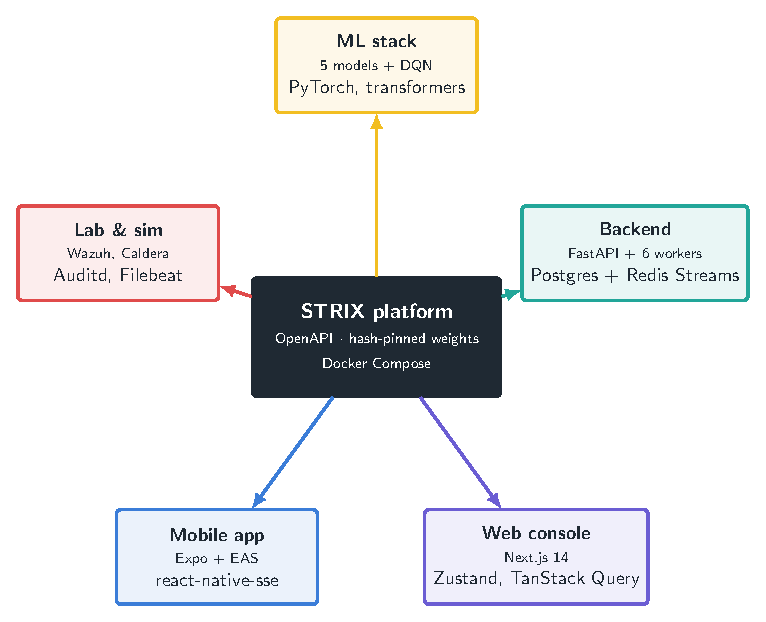
\includegraphics[width=0.55\textwidth]{figures/ch4/diagrams/overview_pillars}
  \caption{The five implementation pillars of CAVIX.}
  \label{fig:ch4:overview}
  \par\medskip
  As figure~\ref{fig:ch4:overview} shows, each one is documented in its own section of this chapter; the central node is the contract every pillar agrees on (an OpenAPI specification, a fixed set of hash-pinned model weights, and a Docker Compose orchestration).
\end{figure}

Four principles drove most of the decisions described below, in order
of priority. First, reproducibility: every Python dependency is
version-pinned, every model weight has a known SHA-256, and the lab
boots from a single shell script. Second, type safety end-to-end: the
Pydantic models behind FastAPI \cite{fastapi2024,pydantic2024} are the
only source of truth for what an alert or a verdict looks like, and
the web and mobile clients consume the generated TypeScript types.
Third, black-box integration of third-party components: every external
dependency (the SIEM, the message bus, the database, each CTI feed)
is consumed through a narrow contract so that replacing one cannot
propagate beyond its own boundary. Fourth, operational maturity of
load-bearing dependencies: a Linux audit subsystem \cite{auditd2024}
that has shipped with the mainline kernel since the 2.6 series, a
Wazuh manager \cite{wazuh2024} already deployed in production SOCs,
and a PostgreSQL database \cite{postgres2024} extended with TimescaleDB
\cite{timescaledb2024} for the time-partitioned detection table.

\section{Hardware and Software Environment}

\subsection{Hardware}

CAVIX targets commodity hardware. Table~\ref{tab:ch4:hardware} lists
the two supported configurations: a development / demonstration
workstation, on which the full Docker \cite{docker2024} Compose
topology runs without a GPU, and an optional training configuration
that benefits from CUDA when one is available. The CPU-only PyTorch
build \cite{paszke2019pytorch} is the default because the CUDA
variant adds roughly three gigabytes to the API image, which is
justified only above the throughput the lab generates. The inference
worker batches up to thirty-two events at a time, a value chosen so
that the per-batch fixed cost of the five-model forward pass is
amortised across enough events to dominate the per-event
serialisation cost, while the batch still drains within the
five-second writer window introduced in section~\ref{sec:integration}.

\begin{table}[H]
  \centering
  \caption{Hardware and software configuration for the two supported
  deployment modes. Neither setup is required to run a jury demo:
  \texttt{jury\_demo.sh} brings up the same Compose topology on any
  machine that can run Docker.}
  \label{tab:ch4:hardware}
  \begin{tabular}{lll}
    \toprule
    \textbf{Resource}    & \textbf{Development / demo}  & \textbf{Training (optional)} \\
    \midrule
    Host                 & x86\_64 workstation          & x86\_64 workstation \\
    CPU                  & 8 cores recommended          & 8+ cores recommended \\
    RAM                  & 16\,GB                       & 16\,GB \\
    GPU                  & None (CPU-only)              & NVIDIA, via \texttt{--device cuda} \\
    Container runtime    & Docker (Compose)             & Docker (Compose) \\
    PyTorch build        & \texttt{torch==2.4.1+cpu}    & \texttt{torch==2.4.1+cu*} \\
    Inference batch size & 32 events                    & not applicable \\
    \bottomrule
  \end{tabular}
\end{table}

\begin{figure}[H]
  \centering
  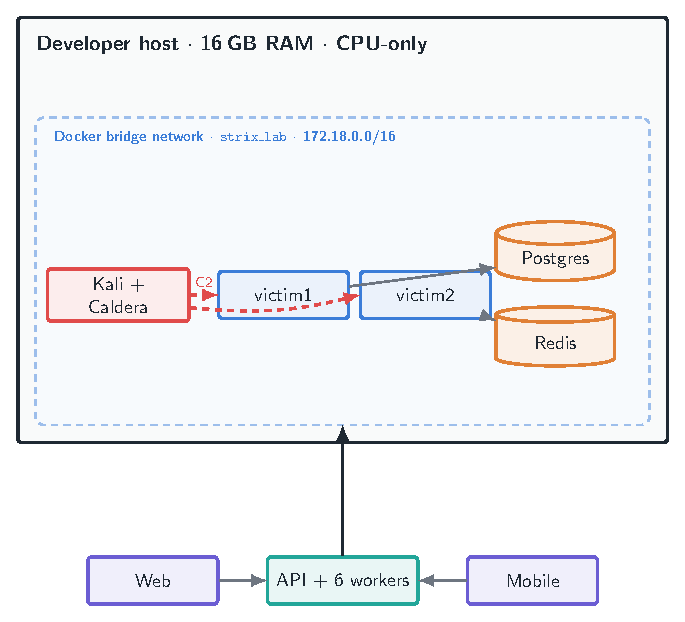
\includegraphics[width=0.78\textwidth]{figures/ch4/diagrams/lab_topology}
  \caption{Lab topology used in this chapter and in chapter~\ref{chap:evaluation} for the evaluation.}
  \label{fig:ch4:topology}
  \par\medskip
  As shown in figure~\ref{fig:ch4:topology}, a single host runs every container: the attacker (Kali with MITRE Caldera \protect\cite{caldera2024}), the two victims with Wazuh agents and \texttt{auditd}, the backing stores (PostgreSQL, Redis) and the user-facing surfaces (API, web, mobile). All containers share the \texttt{172.18.0.0/16} bridge so the attacker can reach the victims directly.
\end{figure}

Two runtime memory budgets matter operationally and are summarised
in table~\ref{tab:ch4:memory}. The inference worker stays around
600\,MB resident under normal load and peaks at roughly 1.2\,GB
during a busy lab run. The Redis \cite{redis2024} memory cap is
deliberately conservative at 512\,MB with a \texttt{noeviction}
policy, so that the writer errors loudly rather than silently
discarding a verdict; because the working-set size scales with
alert volume rather than with a fixed bound, the cap is exposed
through the \texttt{REDIS\_MAXMEMORY} environment variable, and
four gigabytes is sufficient for the longest soak tests we run.

\begin{table}[H]
  \centering
  \caption{Runtime memory budgets for the load-bearing components.}
  \label{tab:ch4:memory}
  \begin{tabular}{llll}
    \toprule
    \textbf{Component}       & \textbf{Default} & \textbf{Tunable via}       & \textbf{Notes} \\
    \midrule
    Inference worker (RSS)   & $\sim$600\,MB    & ---                        & Peaks $\sim$1.2\,GB under attack load \\
    Redis memory cap         & 512\,MB          & \texttt{REDIS\_MAXMEMORY}  & Eviction policy = \texttt{noeviction} \\
    Redis (soak tests)       & 4\,GB            & \texttt{REDIS\_MAXMEMORY}  & Scales with alert volume \\
    \bottomrule
  \end{tabular}
\end{table}

\subsection{Libraries}

The dependencies fall naturally into four stacks that mostly do not
overlap. Splitting them like this also makes it easier to upgrade one
side without disturbing the other. A change to the React Native
\cite{expo2024} version, for example, has no influence on the Python
side except through the OpenAPI contract.

\subsubsection{Backend and machine-learning stack}

\begin{figure}[H]
  \centering
  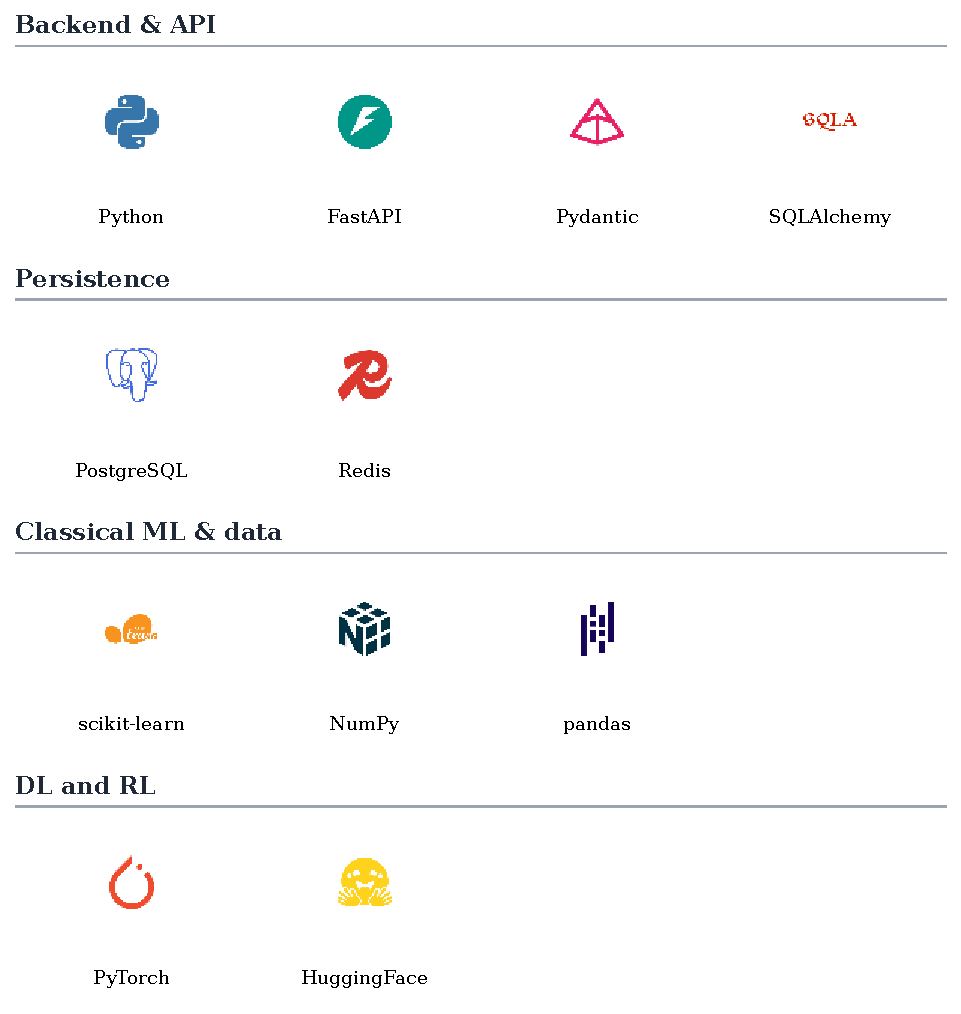
\includegraphics[width=0.78\textwidth]{figures/ch4/logos/stack_logos_backend}
  \caption{Backend and machine-learning libraries, grouped by architectural layer: backend \& API, persistence, classical ML and data tooling, and DL and RL.}
  \label{fig:ch4:logos:backend}
  \par\medskip
  In figure~\ref{fig:ch4:logos:backend}, logos sourced from Simple Icons \protect\cite{simpleicons2024}.
\end{figure}

The backend runs on Python 3.11. FastAPI is the web framework
\cite{fastapi2024}; Pydantic v2 \cite{pydantic2024} handles
validation and is the single source of truth for the OpenAPI
specification consumed downstream by the web and mobile clients.
Persistence is SQLAlchemy 2 \cite{sqlalchemy2024} in its async mode,
backed by \texttt{asyncpg} against a PostgreSQL 16 instance running the
TimescaleDB extension for the time-partitioned \texttt{detections}
hypertable. Job queuing is handled by ARQ \cite{arq2024}, an
asynchronous job-queue library that sits on top of Redis.

For the machine-learning side, PyTorch is the workhorse: every model in
the ensemble (autoencoder, $\beta$-VAE \cite{higgins2017betavae},
Transformer next-stage predictor \cite{vaswani2017attention},
GraphSAGE graph neural network \cite{hamilton2017graphsage}, DQN
policy network \cite{mnih2015dqn}) is a \texttt{torch.nn.Module}. The
graph layers come from PyTorch Geometric \cite{fey2019pyg}. Natural-
language tokens (raw Wazuh log messages and shell commands) are
embedded by SecBERT \cite{secbert2022} through the \texttt{transformers}
library \cite{wolf2020transformers}, then reduced to sixteen
principal components by scikit-learn before joining the rest of the
feature vector.

A few smaller dependencies do important load-bearing work and are worth
naming. \texttt{argon2-cffi} \cite{biryukov2016argon2} hashes
operator passwords. \texttt{pybreaker} wraps every outgoing call to an
external API in a circuit breaker so a transient URLhaus outage does
not back-pressure the rest of the platform. \texttt{structlog},
\texttt{prometheus-client} and \texttt{opentelemetry-sdk}
\cite{prometheus2024,opentelemetry2024} cover the three observability
pillars (structured logs, metrics, traces).

\subsubsection{Reinforcement-learning training stack}

The training pipeline under \texttt{RL\_agent/} reuses the fused DL+RL
toolkit shown in figure~\ref{fig:ch4:logos:backend} and is intentionally
simpler than the inference path. It pulls in PyTorch for the network,
NumPy and pandas for tensor and tabular operations, scikit-learn for the
balanced-threshold search, OpenAI Gym for the \texttt{APTEnv} base class,
and Matplotlib for the diagnostic plots that come out of every training
run. There is no FastAPI here, no database, no asynchronous code; the
training is a long-running CPU loop that reads a few thousand carved
attack sequences and writes a checkpoint into \texttt{RL\_agent/outputs/}.

\subsubsection{Web console}

\begin{figure}[H]
  \centering
  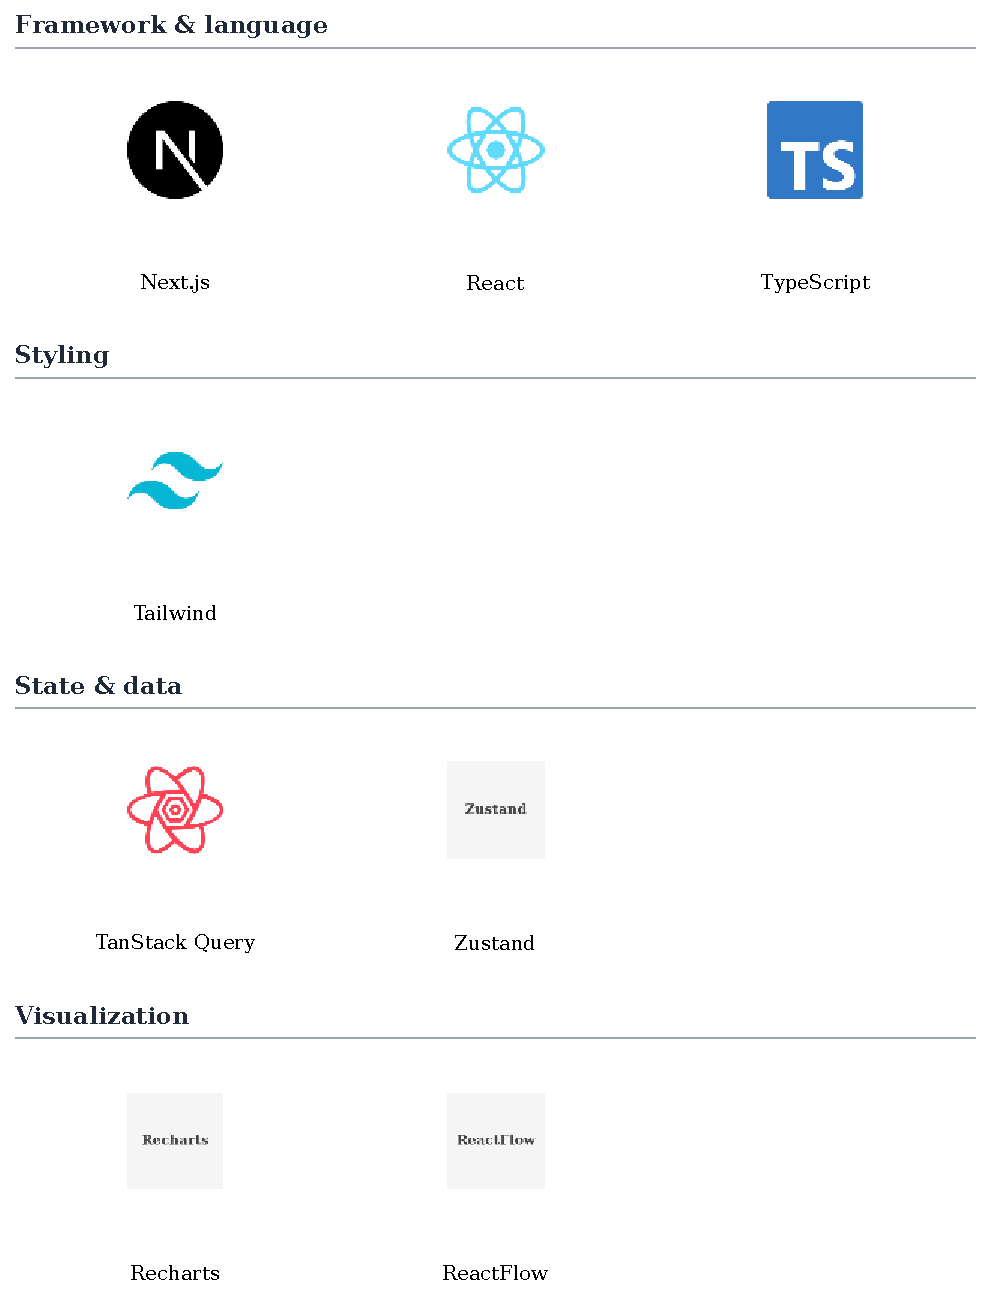
\includegraphics[width=0.70\textwidth]{figures/ch4/logos/stack_logos_web}
  \caption{Web-console stack, grouped by role: framework and language, styling, and state and data.}
  \label{fig:ch4:logos:web}
  \par\medskip
  Figure~\ref{fig:ch4:logos:web} shows only the libraries published by Simple Icons. Zustand, Recharts, and ReactFlow are also part of the production build but lack a Simple Icons entry and are omitted from the grid; they are described in the prose below.
\end{figure}

The analyst console is a Next.js 14 application using the App Router
\cite{nextjs2024}. Server-side state is managed by TanStack Query;
client-side state by Zustand. Tailwind CSS gives us a single utility
language for styling. Recharts and ReactFlow cover the two distinct
visualization styles we need: time-series telemetry on one side, the
host/process graph rendered with a force-directed layout on the other.
Generated API types come from \texttt{openapi-typescript}: the build
fails if the TypeScript bindings drift away from the backend's actual
OpenAPI specification.

\subsubsection{Mobile companion}

\begin{figure}[H]
  \centering
  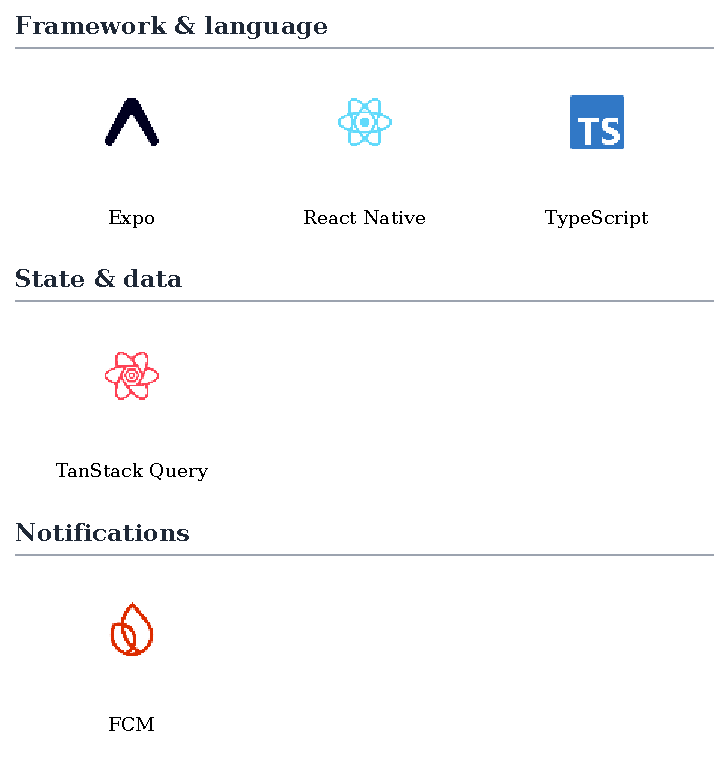
\includegraphics[width=0.62\textwidth]{figures/ch4/logos/stack_logos_mobile}
  \caption{Mobile-application stack, grouped by role: framework and language, state and data, and notifications.}
  \label{fig:ch4:logos:mobile}
  \par\medskip
  Figure~\ref{fig:ch4:logos:mobile} captures the following. Expo provides the dev-client build pipeline; Expo Push (no Simple Icons entry, omitted from the grid) handles notifications, with a fall-back path to Firebase Cloud Messaging where Expo's service is not available.
\end{figure}

The mobile application is React Native through Expo SDK 54
\cite{expo2024}. The dev-client build pipeline gives us native modules
without the burden of maintaining a custom iOS or Android project.
Push notifications go through Expo Push rather than bare Firebase
Cloud Messaging because Expo Push offers a single delivery surface
across iOS and Android, removing the need for separate APNs
provisioning on Apple devices while still routing through the same
FCM infrastructure on Android. Data fetching, store layout, and the
OpenAPI-derived types are mirrored from the web side, which means
the two clients share an intuitive mental model even though they
share no actual code.

\subsection{Development Tools}

Both halves of the codebase have a single quality gate. On the Python
side, \texttt{ruff} is the linter and formatter (targeting Python 3.11,
line length one hundred), \texttt{mypy --strict} is the type checker,
\texttt{pytest} is the test runner, and \texttt{hypothesis} and
\texttt{schemathesis} drive property-based tests against the OpenAPI
schema. On the TypeScript side, \texttt{eslint} and \texttt{tsc}
handle the same job. The web build also enforces a \texttt{check:api-
types} command that fails the pipeline if the generated TypeScript
types are out of date with the backend's OpenAPI specification.
This is how we prevent the most common form of backend--frontend
drift, where a renamed field passes the type checker on each side
in isolation but produces a runtime error in production.

\begin{figure}[H]
  \centering
  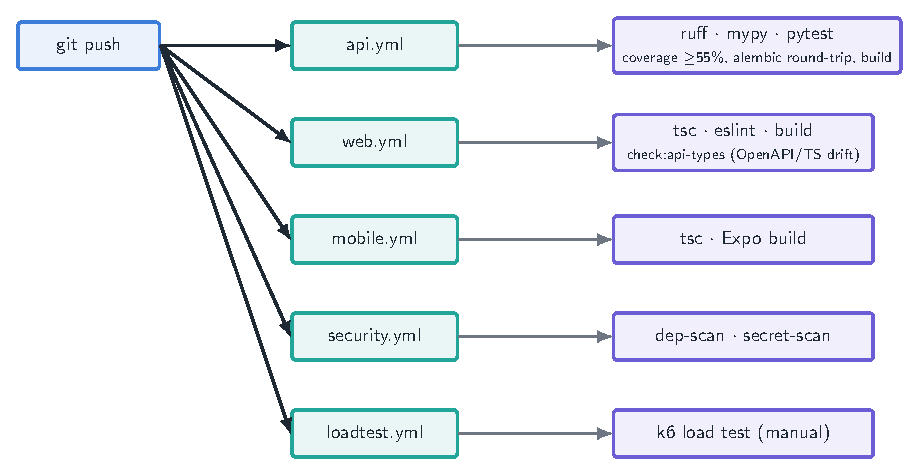
\includegraphics[width=0.95\textwidth]{figures/ch4/diagrams/ci_pipeline}
  \caption{Continuous-integration pipeline.}
  \label{fig:ch4:ci}
  \par\medskip
  As depicted in figure~\ref{fig:ch4:ci}, a single push triggers five parallel GitHub Actions workflows: \texttt{api.yml} (backend tests against real PostgreSQL and Redis service containers), \texttt{lint.yml} (Ruff + mypy on the Python tree), \texttt{web.yml} (TypeScript compile, ESLint, and the \texttt{check:api-types} gate), \texttt{mobile.yml} (Expo prebuild + Jest), and \texttt{models.yml} (model-artefact hash verification). The \texttt{api.yml} job runs against real service containers rather than mocks to ensure that Alembic migrations, which mocked tests cannot exercise, are validated on every push.
\end{figure}

\begin{figure}[H]
  \centering
  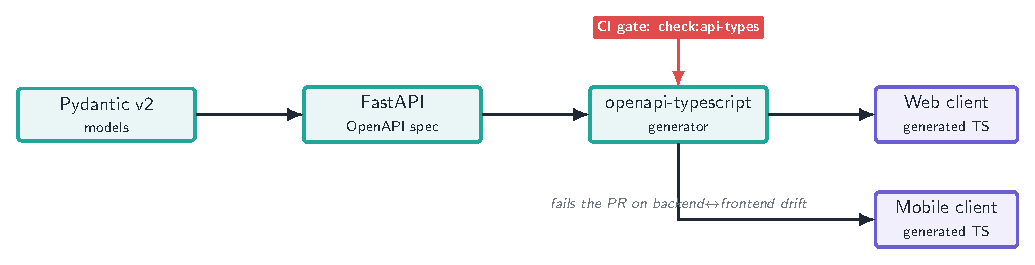
\includegraphics[width=0.85\textwidth]{figures/ch4/diagrams/type_safety_chain}
  \caption{The type-safety chain from Pydantic to the two clients.}
  \label{fig:ch4:typesafety}
  \par\medskip
  As figure~\ref{fig:ch4:typesafety} shows, the CI gate at the centre is what catches silent drift between the backend and the frontends.
\end{figure}

The container images themselves are built from \texttt{python:3.11-slim}
for everything Python and \texttt{node:20-bookworm-slim} for the web
build. Both use multi-stage builds so the final runtime layer does not
carry the compiler toolchain. The Compose stacks live under
\texttt{infra/} (six of them, each scoped to a specific concern:
API, lab, victim, simulation, chaos, platform-deps), and there is a
\texttt{Procfile.host} for the alternative workflow where the API and
workers run directly on the developer's machine under Honcho rather
than inside Docker.

\section{Dataset Selection and Justification}
% TODO: criteria-driven dataset selection rationale.

\subsection{Selection Criteria}
% TODO

\subsection{Elimination Process}
% TODO

\subsection{Final Selection}
% TODO

\section{Dataset Description}

\subsection{Linux APT Dataset 2024}

The training data comes from a single source: the Linux APT
intrusion-detection dataset published in 2024 by Karim, Afzal, Iqbal
and Al Abri in \emph{Data in Brief} \cite{karim2024linux}. Their
collection setup matches what CAVIX targets very closely: a Kali
attacker host emulating four real-world APT actors (APT41, APT28,
APT29 and Turla) against three Ubuntu 22.04 victims, with a Wazuh 4.5.2
manager collecting alerts and Kaspersky Security Center 14.2 acting as
a complementary endpoint sensor. The collection ran for fourteen weeks,
between October 2023 and January 2024.

\begin{figure}[H]
  \centering
  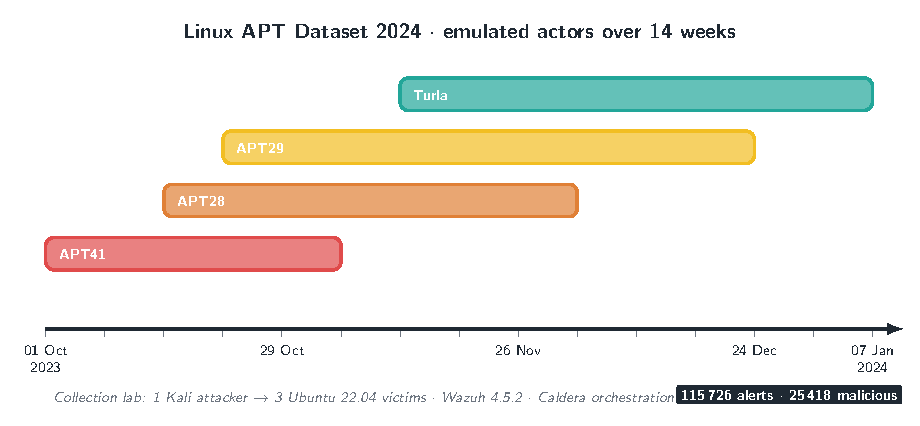
\includegraphics[width=0.95\textwidth]{figures/ch4/diagrams/dataset_timeline}
  \caption{The 14-week collection window of the Linux APT Dataset 2024.}
  \label{fig:ch4:timeline}
  \par\medskip
  As shown in figure~\ref{fig:ch4:timeline}, the four APT campaigns overlap in time; this is deliberate in the original paper, since real APT activity rarely happens in a serialised, mutually-exclusive schedule.
\end{figure}

We materialise the dataset inside CAVIX as two parquet files under
\texttt{apps/models/} (all repository paths in this chapter are
relative to the monorepo root): a feature matrix with 115\,726 rows
by 119 columns (\texttt{feature\_matrix\_no\_leakage.parquet}), and
an alignment table with the binary label and the cyber-kill-chain
stage encoded as integers (\texttt{labels.parquet}). Both files are
the output of the preprocessing pipeline whose
\emph{conceptual} design is given in chapter~\ref{chap:conception}
and whose \emph{implementation} is described in
section~\ref{sec:preprocessing} of this chapter. They are versioned
in the repository, which means a fresh checkout reproduces the exact
training run that produced the shipped model weights.

\subsection{Statistics}

\begin{figure}[H]
  \centering
  \begin{minipage}[c]{0.40\textwidth}
    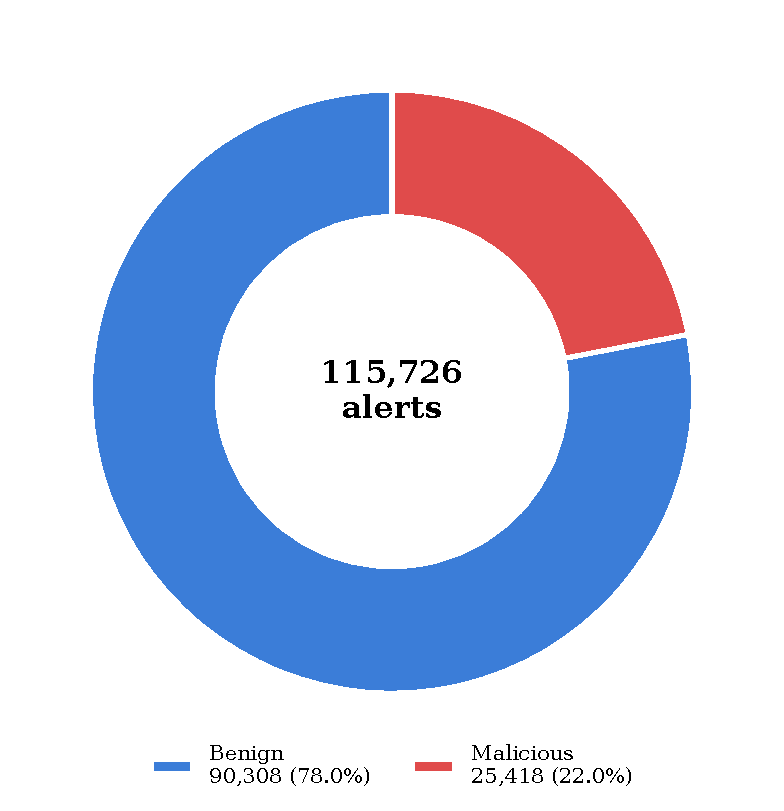
\includegraphics[width=\textwidth]{figures/ch4/charts/dataset_class_split}
  \end{minipage}\hfill
  \begin{minipage}[c]{0.58\textwidth}
    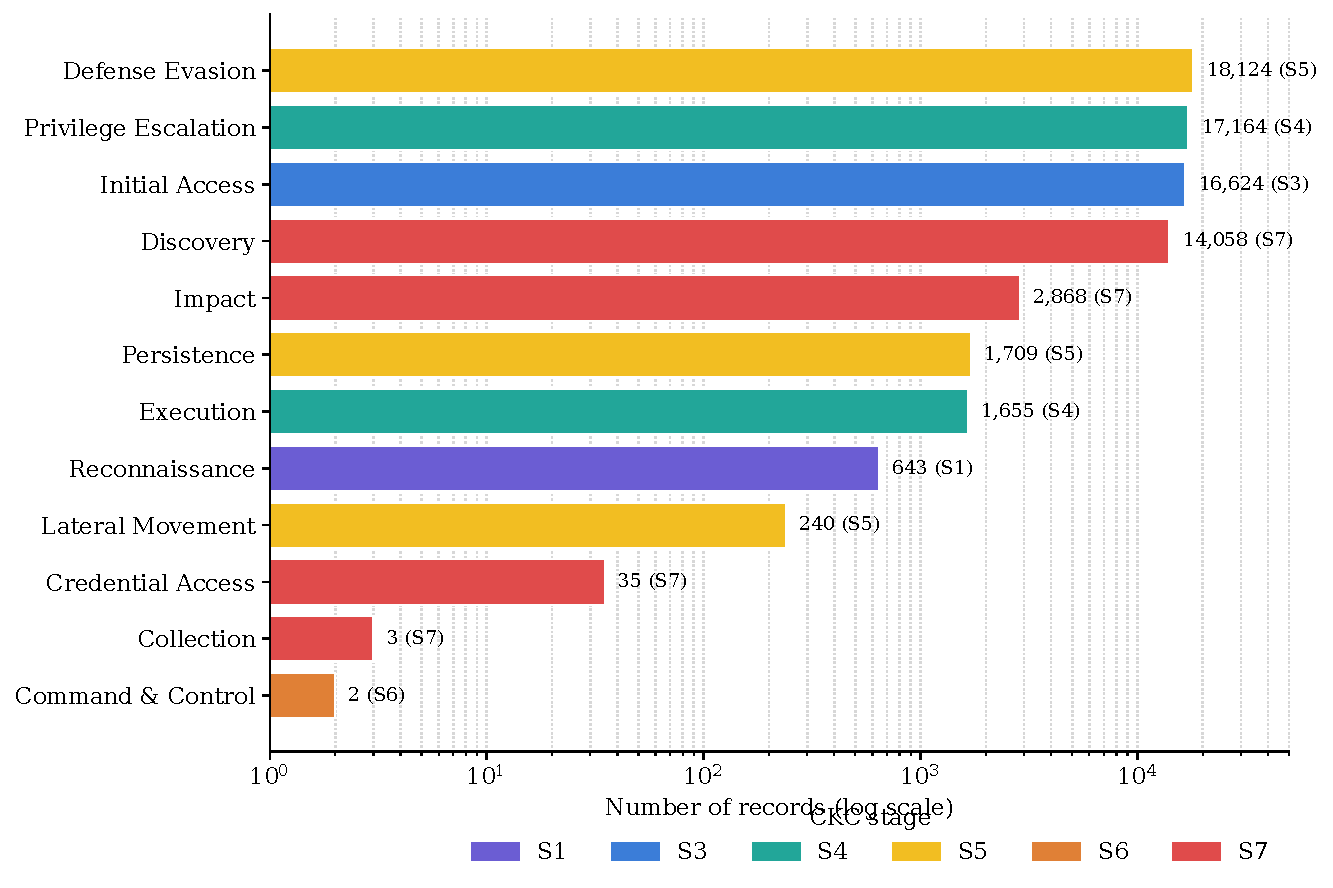
\includegraphics[width=\textwidth]{figures/ch4/charts/dataset_tactic_bars}
  \end{minipage}
  \caption{Class distribution and per-tactic distribution.}
  \label{fig:ch4:datasetstats}
  \par\medskip
  In figure~\ref{fig:ch4:datasetstats}, the binary split (left) is twenty-two percent malicious, which is generous compared to the typical SIEM signal-to-noise ratio. The per-tactic distribution (right) is skewed: Defense Evasion, Privilege Escalation and Initial Access together account for roughly half of the labelled malicious alerts, while Weaponization (S2) and Command \& Control (S6) are effectively absent.
\end{figure}

The skew at the tail of figure \ref{fig:ch4:datasetstats} matters. With
only two C\&C events and zero Weaponization events in the entire
training set, the Transformer's output heads for those two CKC stages
cannot learn anything meaningful. We deal with this in two places: at
training time, by setting the class weights of S2 and S6 to zero in
the cross-entropy loss (whose formulation is given in
chapter~\ref{chap:conception} together with the rest of the
Transformer's training objective), and at inference time, by adding
a deterministic gate in front of the DQN that refuses to fire an
intervention purely on the basis of a low-confidence S2 or S6
prediction. We expand on this gate in section
\ref{sec:integration}.

The 55-column feature vector consumed by every model is the
concatenation of three blocks: twenty-three individual features (binary
indicators, location flags, four numeric quantities), sixteen
principal components of the SecBERT embedding of the raw log message,
and sixteen principal components of the SecBERT embedding of the shell
command. The component count of sixteen on each text branch was
chosen as the smallest value that retains above 95\,\% of the
variance on at least one branch while keeping the embedding's
contribution to the 55-dimensional vector roughly balanced against
the twenty-three structured features. The variance retained by the
PCA reduction is 77.82\,\% on the log side and 97.05\,\% on the
command side; we attribute this asymmetry to the narrower lexical
distribution of shell commands relative to the multi-source log
messages, although the precise type--token ratio of the two corpora
is not measured here.

\begin{figure}[H]
  \centering
  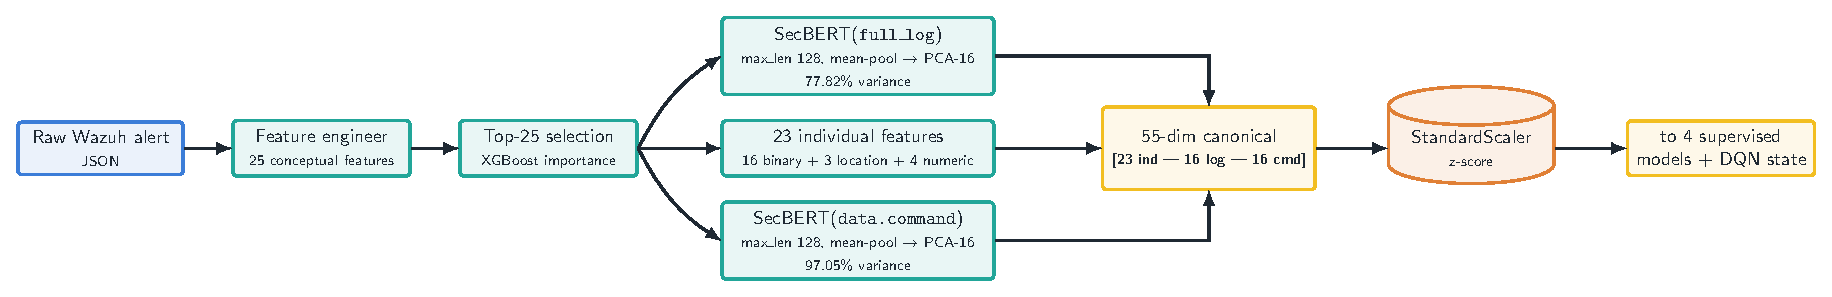
\includegraphics[width=\textwidth]{figures/ch4/diagrams/feature_pipeline}
  \caption{Feature pipeline from raw Wazuh alert to the 55-dimensional vector consumed by every downstream model.}
  \label{fig:ch4:featurepipeline}
  \par\medskip
  As illustrated in figure~\ref{fig:ch4:featurepipeline}, the two SecBERT branches are responsible for embedding the unstructured text fields; the central twenty-three-feature stream carries the structured signals.
\end{figure}

Every artefact in this pipeline is content-addressed. The selected-
features manifest, the standard scaler, both SecBERT PCA bases, the
probability calibrators, and the GNN metadata bundle are all listed in
\texttt{apps/models/registry.json} (registry version 4) together with
their SHA-256 digests. The inference worker refuses to start if any of
those hashes drift away from the manifest, a safeguard we added
after an accidental notebook re-run had once silently overwritten the
calibrator and shifted every $\beta$-VAE malicious-probability by a
few percent.

\subsection{Simulated APT Groups}

\begin{figure}[H]
  \centering
  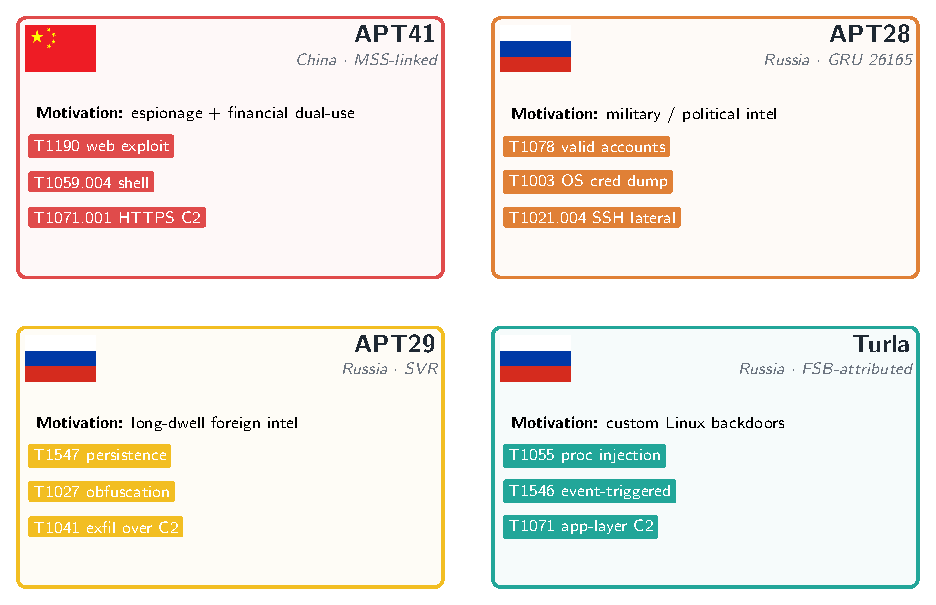
\includegraphics[width=0.78\textwidth]{figures/ch4/diagrams/apt_groups_cards}
  \caption{The four APT groups emulated in the Linux APT Dataset 2024 \protect\cite{karim2024linux}.}
  \label{fig:ch4:aptgroups}
  \par\medskip
  As depicted in figure~\ref{fig:ch4:aptgroups}, the TTP rows are drawn from MITRE ATT\&CK \protect\cite{mitre_attack} and reflect the techniques the paper's authors actually exercised against the Ubuntu victims; the country flags are sourced from a public flag CDN.
\end{figure}

APT41 is a Chinese threat actor with a documented dual-use posture
(state-sponsored espionage alongside financially motivated intrusions).
APT28, APT29 and Turla are all Russian, attributed respectively to the
GRU, the SVR and the FSB. Three of the four cards in
figure \ref{fig:ch4:aptgroups} carry the same flag because the
attributed-actor distribution during the dataset's collection window
skews that way; this is not a sampling artefact. The TTPs listed under each card are
specifically those exercised by the dataset authors against the
victims; they are not a generic summary of each group's full
arsenal.

\section{Data Preprocessing Pipeline}
\label{sec:preprocessing}
% TODO

\subsection{CSV Repair}
% TODO

\subsection{Field Extraction and MITRE Filtering}
% TODO

\subsection{Timestamp Parsing and Chronological Sorting per Agent}
% TODO

\subsection{Attack Sequence Graph Construction}
% TODO

\subsection{Attack Pattern Analysis}
% TODO

\subsection{Exported Artifacts}
% TODO

\section{Feature Engineering}
% TODO

\subsection{Phase 1}
% TODO

\subsection{Phase 2}
% TODO

\subsection{SecBERT Embedding}
% TODO

\subsection{Feature Selection with XGBoost/RandomForest}
% TODO

\section{Attack Simulation with MITRE Caldera}
\label{sec:caldera}

\subsection{Why Caldera}

The dataset above tells us what attackers do; Caldera lets us replay
that behaviour against our own infrastructure on demand
\cite{caldera2024}. Three roles emerge for it inside CAVIX. First, it
is a sanity-check that the dataset's distributional shape generalises
to a fresh deployment of our platform: if we run an APT29 adversary
profile against a clean Wazuh deployment and the resulting alert volume
is wildly different from what the dataset contains, something in our
pipeline is wrong. Second, Caldera is a regression harness: every
change to the rules, the workers, or a model weight is validated by
re-running the same nine-tactic scenario and diffing the per-tactic
detection report against the previous build. Third, it is a demo
driver, used by \texttt{jury\_demo.sh} to produce a deterministic
attack story stakeholders can follow live on the web console.

\begin{figure}[H]
  \centering
  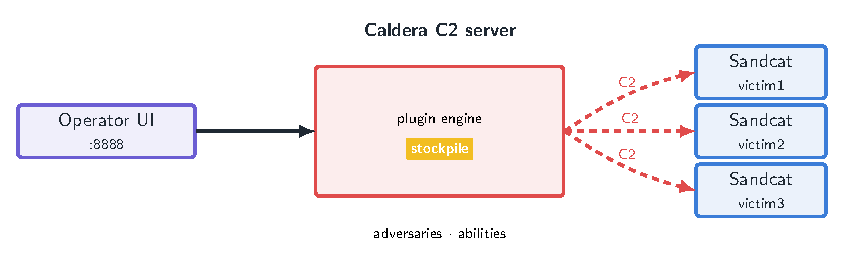
\includegraphics[width=0.85\textwidth]{figures/ch4/diagrams/caldera_architecture}
  \caption{Caldera's deployment shape: an operator-facing web interface
  on port 8888, a C2 server that pushes abilities to Sandcat agents
  deployed on each victim, and an internal stockpile of adversaries
  (sequences of abilities) and abilities (individual TTPs).}
  \label{fig:ch4:calderaarch}
\end{figure}

\subsection{Caldera Deployment}

We bring Caldera up from source in a Docker container. The build
arguments and runtime configuration live under
\texttt{infra/lab-provisioning/01-attacker-caldera.sh}. The container
exposes five ports, listed in figure \ref{fig:ch4:calderaports}. Of
these, only the operator UI on 8888 is published to the host; the
four C2 ports are reachable only by the Sandcat agents on the same
Docker bridge network. Persistent state (\texttt{persist/conf/} and
\texttt{persist/data/}) is mounted from the host, which means
operations and credentials survive a container rebuild. The operator
password is rotated automatically by a small PyYAML patch applied
during \texttt{docker run} so that the deployment does not run with
the documented sample credentials from the upstream
configuration \cite{caldera2024}.

\begin{figure}[H]
  \centering
  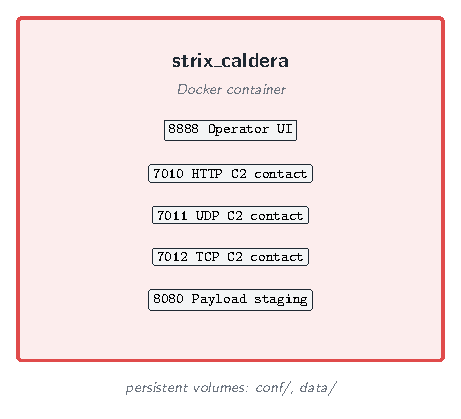
\includegraphics[width=0.45\textwidth]{figures/ch4/diagrams/caldera_ports}
  \caption{Port assignments inside the \texttt{strix\_caldera} container.}
  \label{fig:ch4:calderaports}
\end{figure}

\subsection{The Nine Paper-Aligned Tactics}

Caldera comes with an extensive stockpile, but the runner in
\texttt{infra/scripts/lab\_simulate.sh} restricts itself to the nine
tactics that the Linux APT Dataset 2024 covers, in roughly
the order an APT campaign goes through them
\cite{karim2024linux,mitre_attack}. Reconnaissance is the only tactic
that does not actually go through Caldera; we drive it from a small
shell script (\texttt{recon\_burst.sh}) because Caldera's ability
model assumes a delivered Sandcat implant on the target, and
Reconnaissance by definition targets a host \emph{before} any
implant is dropped.

\begin{figure}[H]
  \centering
  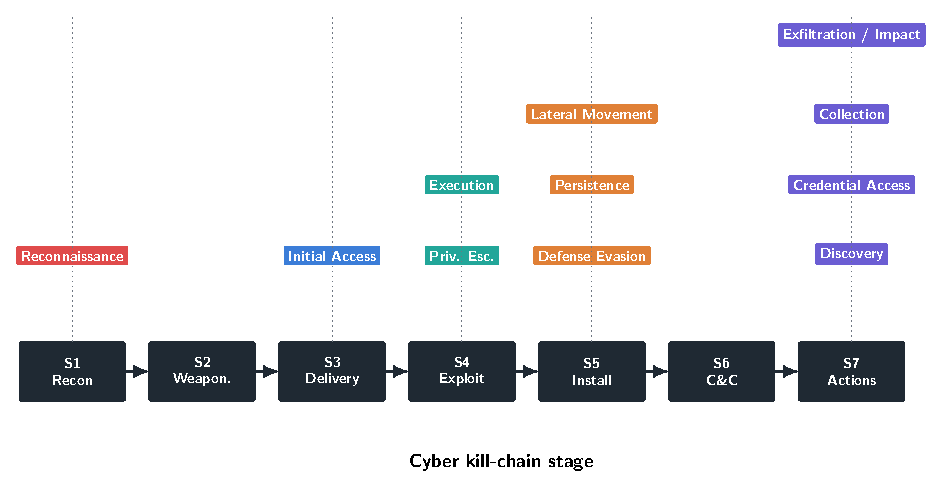
\includegraphics[width=\textwidth]{figures/ch4/diagrams/nine_tactics_kcc}
  \caption{The nine tactics overlaid on the seven-stage Cyber Kill Chain.}
  \label{fig:ch4:9tactics}
  \par\medskip
  As figure~\ref{fig:ch4:9tactics} shows, multiple tactics map to the same stage (Lateral Movement and Persistence both anchor on Installation (S5), for instance) because the kill chain is coarser than ATT\&CK.
\end{figure}

\subsection{Topology Discovery and the Run Manifest}

Before any tactic fires, the runner inspects the live Compose stack
and emits a JSON manifest of what it found. The manifest is the only
ground truth a downstream report has access to: it pins the attacker's
IP, the victims' IPs and hostnames, the agents that were online when
the run started, and the planned tactic chain.

\begin{figure}[H]
  \centering
  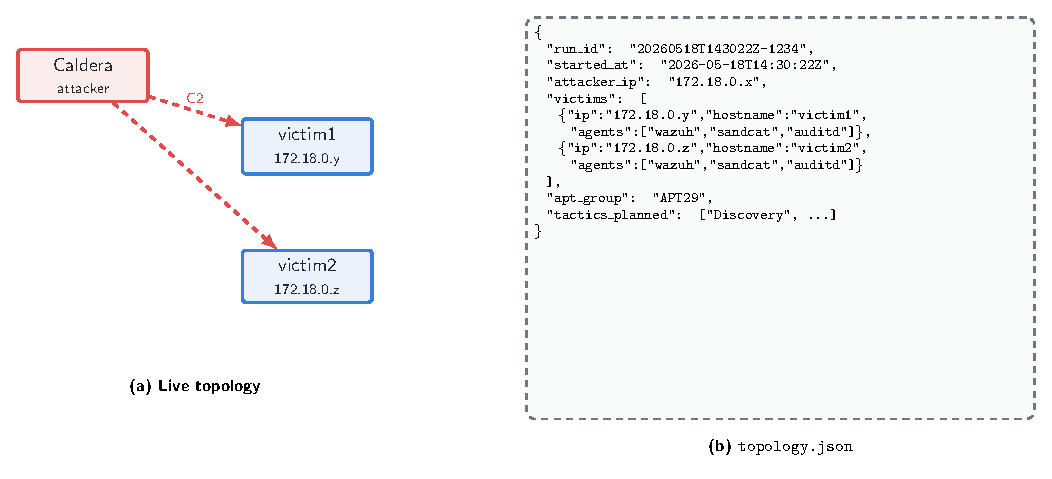
\includegraphics[width=0.95\textwidth]{figures/ch4/diagrams/topology_run_manifest}
  \caption{Live topology (left) and the \texttt{topology.json} that records it (right).}
  \label{fig:ch4:manifest}
  \par\medskip
  As shown in figure~\ref{fig:ch4:manifest}, every run writes its own manifest under \texttt{infra/simulation/runs/\{RUN\_ID\}/}; the chapter-6 evaluation joins these manifests with the database verdicts to compute per-victim metrics.
\end{figure}

\subsection{Per-Tactic and Final Reports}

The orchestrator \texttt{run\_full\_simulation.py} loops through the
planned tactic chain. For each tactic it captures a baseline of
platform counters, fires the Caldera operation, waits a dwell period
for the alert-to-verdict pipeline to drain, and prints a delta. At
the end of the run it also prints an aggregate report with the
wallclock duration, the resolution outcome of each tactic (link
return codes, alert deltas, CKC-stage deltas), the distribution of
DQN actions that fired, and the histogram of Wazuh rule IDs that hit
in the run window.

\begin{figure}[H]
  \centering
  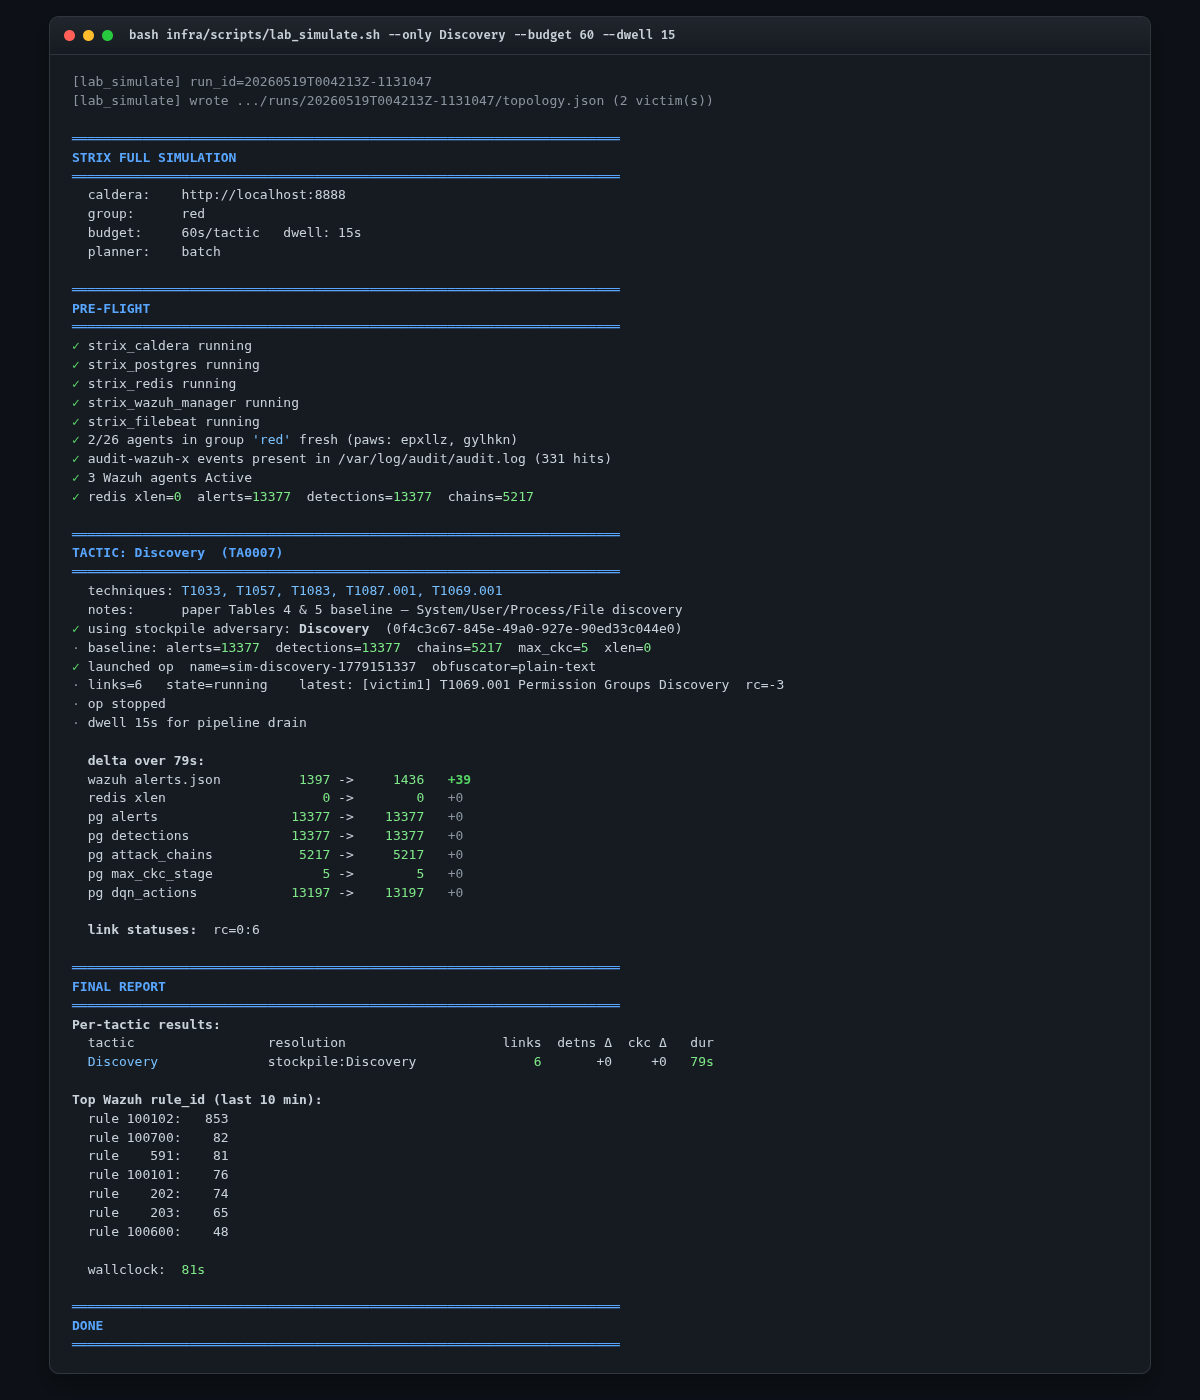
\includegraphics[width=0.78\textwidth]{figures/ch4/screenshots/per_tactic_report}
  \caption{Live output of a Discovery-only run captured during the writing of this chapter (\texttt{bash infra/scripts/lab\_simulate.sh --only Discovery --budget 60 --dwell 15}).}
  \label{fig:ch4:pertacticreport}
  \par\medskip
  In figure~\ref{fig:ch4:pertacticreport}, the pre-flight section asserts every dependency is up; the per-tactic section records the platform delta over the 79-second run; the final report aggregates across the whole tactic chain (here, just one tactic).
\end{figure}

\customwarning{The auditd rules under
\texttt{/etc/audit/rules.d/strix.rules} are persisted across host
reboots, but the kernel may load them in a different order after a
restart. \texttt{lab\_simulate.sh} validates the load with
\texttt{sudo auditctl -l | grep audit-wazuh-x} before launching the
first tactic. If that check fails, run
\texttt{sudo augenrules --load} and try again.}

\begin{figure}[H]
  \centering
  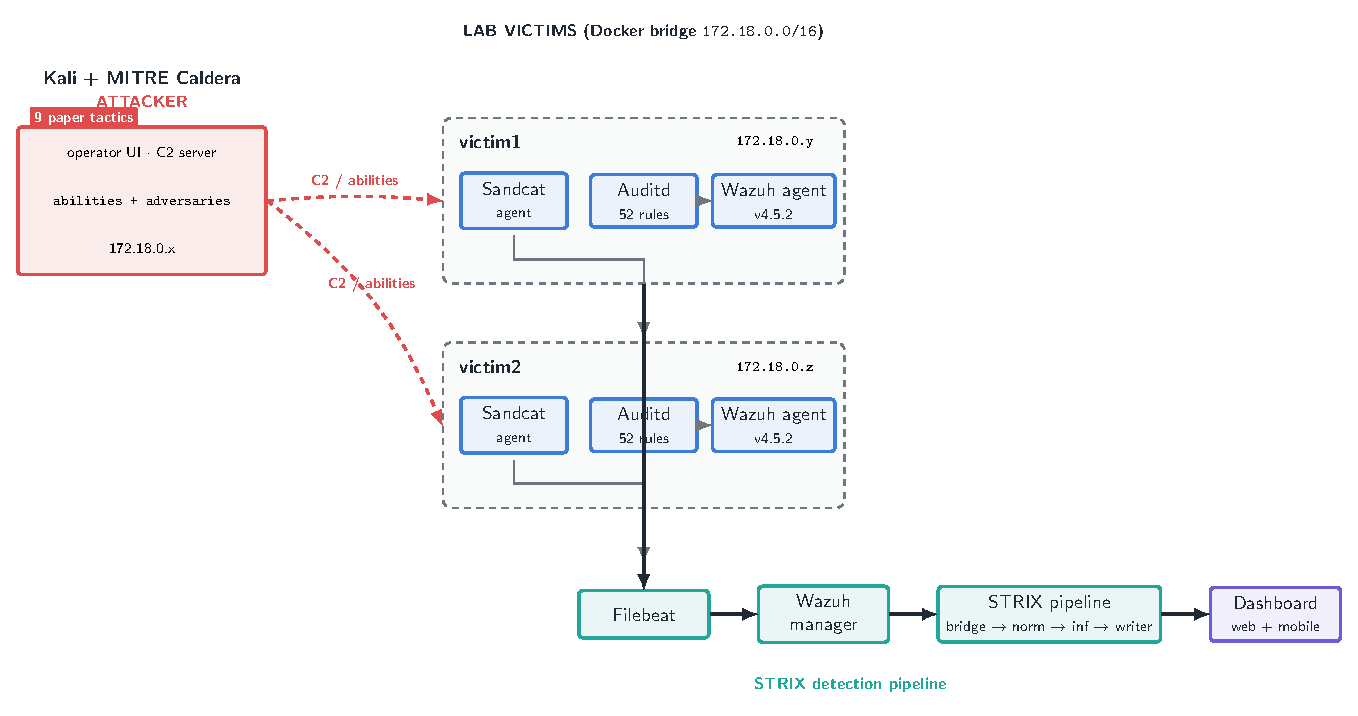
\includegraphics[width=\textwidth]{figures/ch4/diagrams/simulation_envir}
  \caption{The simulation environment as a single picture.}
  \label{fig:ch4:simenv}
  \par\medskip
  As illustrated in figure~\ref{fig:ch4:simenv}, the attacker on the left issues C2 abilities through Caldera; each victim runs a Sandcat agent, the host \texttt{auditd}, and a Wazuh agent. The bottom row is the CAVIX detection pipeline that consumes the resulting telemetry. Every other diagram in this chapter is a zoom-in on one part of this figure.
\end{figure}

\section{Platform Description}
\label{sec:platform}

\subsection{Wazuh SIEM}

We deliberately did not modify the Wazuh manager binary. Instead, the
manager runs upstream and CAVIX adds three things on top of it: a set
of auditd rules tuned for the Linux kill chain
\cite{auditd2024,karim2024linux}, a local rule file deployed at
\texttt{/var/ossec/etc/rules/local\_rules.xml}, and a muting hierarchy
that silences the noisy parent rules while keeping a small number of
high-value custom rules audible.

\begin{figure}[H]
  \centering
  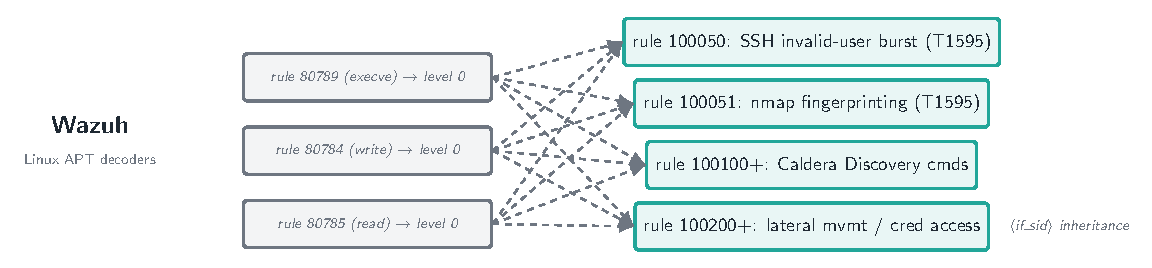
\includegraphics[width=0.95\textwidth]{figures/ch4/diagrams/wazuh_logo_rules}
  \caption{Custom Wazuh rule hierarchy.}
  \label{fig:ch4:wazuhrules}
  \par\medskip
  As depicted in figure~\ref{fig:ch4:wazuhrules}, parent rules 80789, 80784 and 80785 are forced to \texttt{level=0} so they do not flood the alert stream; the child rules 100050, 100051, 100100+ and 100200+ inherit through \texttt{$\langle$if\_sid$\rangle$} and only fire when the parent matches a specific attacker pattern.
\end{figure}

Two of the custom rules deserve a mention. Rule 100050 fires on a
burst of \texttt{sshd} invalid-user attempts and rule 100051 on a
short-window port scan; both are mapped to T1595 in MITRE ATT\&CK
\cite{mitre_attack}, which puts them at Reconnaissance, the first
stage of the kill chain, where signature-based SIEMs typically have
nothing to say. Catching anything at this stage is the difference
between an "early-detection" platform and a "post-mortem" platform,
and these two rules are how we get there.

The Wazuh manager writes alerts as newline-delimited JSON to
\texttt{/var/ossec/logs/alerts/alerts.json}. From the CAVIX side, that
file is the only contract with Wazuh: everything downstream is owned
by us, which makes it easy to swap Wazuh out for another SIEM
without rewriting the detection pipeline.

\subsection{Auditd \texorpdfstring{$\rightarrow$}{->} Filebeat Ingestion}

The actual kernel-level signal comes from \texttt{auditd}, configured
through 52 rules grouped by CKC phase in
\texttt{infra/auditd/strix.rules}. The rule count is not arbitrary:
it is the union of the kernel-syscall watchpoints needed to capture
the nine MITRE-aligned tactics introduced in section~\ref{sec:caldera}
(roughly five to six watchpoints per tactic, depending on whether
the tactic touches file, process, or attribute primitives). The
rules use the Wazuh naming convention (\texttt{audit-wazuh-x} for
execve, \texttt{audit-wazuh-w} for write, \texttt{audit-wazuh-r}
for read, \texttt{audit-wazuh-a} for attribute changes) so the Wazuh
manager picks them up without further configuration. Installation
is a two-step affair documented in the script header:

\begin{verbatim}
sudo cp infra/auditd/strix.rules /etc/audit/rules.d/strix.rules
sudo augenrules --load
sudo auditctl -l | grep audit-wazuh-x   # validation
\end{verbatim}

\begin{figure}[H]
  \centering
  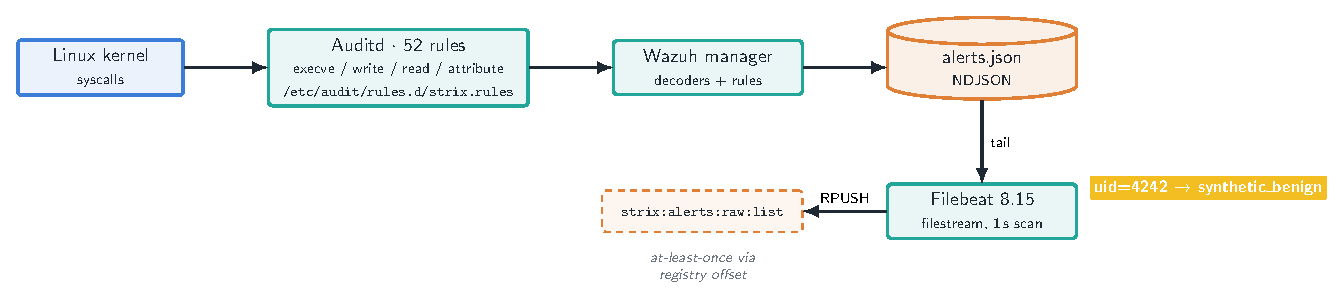
\includegraphics[width=0.98\textwidth]{figures/ch4/diagrams/auditd_filebeat_flow}
  \caption{From kernel syscalls to the Redis ingest list.}
  \label{fig:ch4:auditdflow}
  \par\medskip
  Figure~\ref{fig:ch4:auditdflow} captures the following. Filebeat \protect\cite{filebeat2024} tails Wazuh's \texttt{alerts.json} with a one-second check interval and pushes each line into the Redis staging list. The Filebeat registry guarantees at-least-once delivery: if Redis dies, the offset is not advanced and Filebeat resumes from the last successful push on recovery.
\end{figure}

We chose Filebeat over heavier alternatives such as Logstash or
Fluentd because the shipper sits on the victim host: a Go binary
with a sub-50\,MB resident footprint and a single registry file is
operationally cheaper to deploy at scale than a JVM-based shipper,
and the at-least-once delivery semantics required from the shipper
are already provided by the registry without an external broker.

A small JavaScript processor on Filebeat tags events from UID 4242,
the \texttt{strixbenign} user under which the benign-traffic generator
\texttt{infra/simulation/benign\_traffic.py} runs, with
\texttt{strix.synthetic\_benign=true}. The generator issues a
randomised mix of routine shell, file, and network activity against
the victim hosts and is started by \texttt{lab\_simulate.sh}
alongside the attack tactics; its purpose is to give the test set a
realistic ratio of benign to malicious traffic so that the
false-positive rate is measured against representative noise. The
downstream workers honour the tag and filter the synthetic traffic
out of the metrics the dashboard reports, while still feeding it
through the model layer.

\subsection{Backend Integration: Workers and Redis Streams}
\label{sec:integration}

This is the heart of the platform: a five-stage pipeline that turns a
raw Wazuh JSON line into a database row, an SSE event, and possibly a
mobile push notification, in less than two seconds on the developer's
laptop. Figure~\ref{fig:ch4:components} shows the static
decomposition of the backend, the FastAPI routes, services, repos,
adapters, workers, model artefacts, and observability that section
3.7.3 of the conception chapter described at the four-component level.
Figure~\ref{fig:ch4:dataflowmaster} then traces the runtime flow
through it.

\begin{figure}[H]
  \centering
  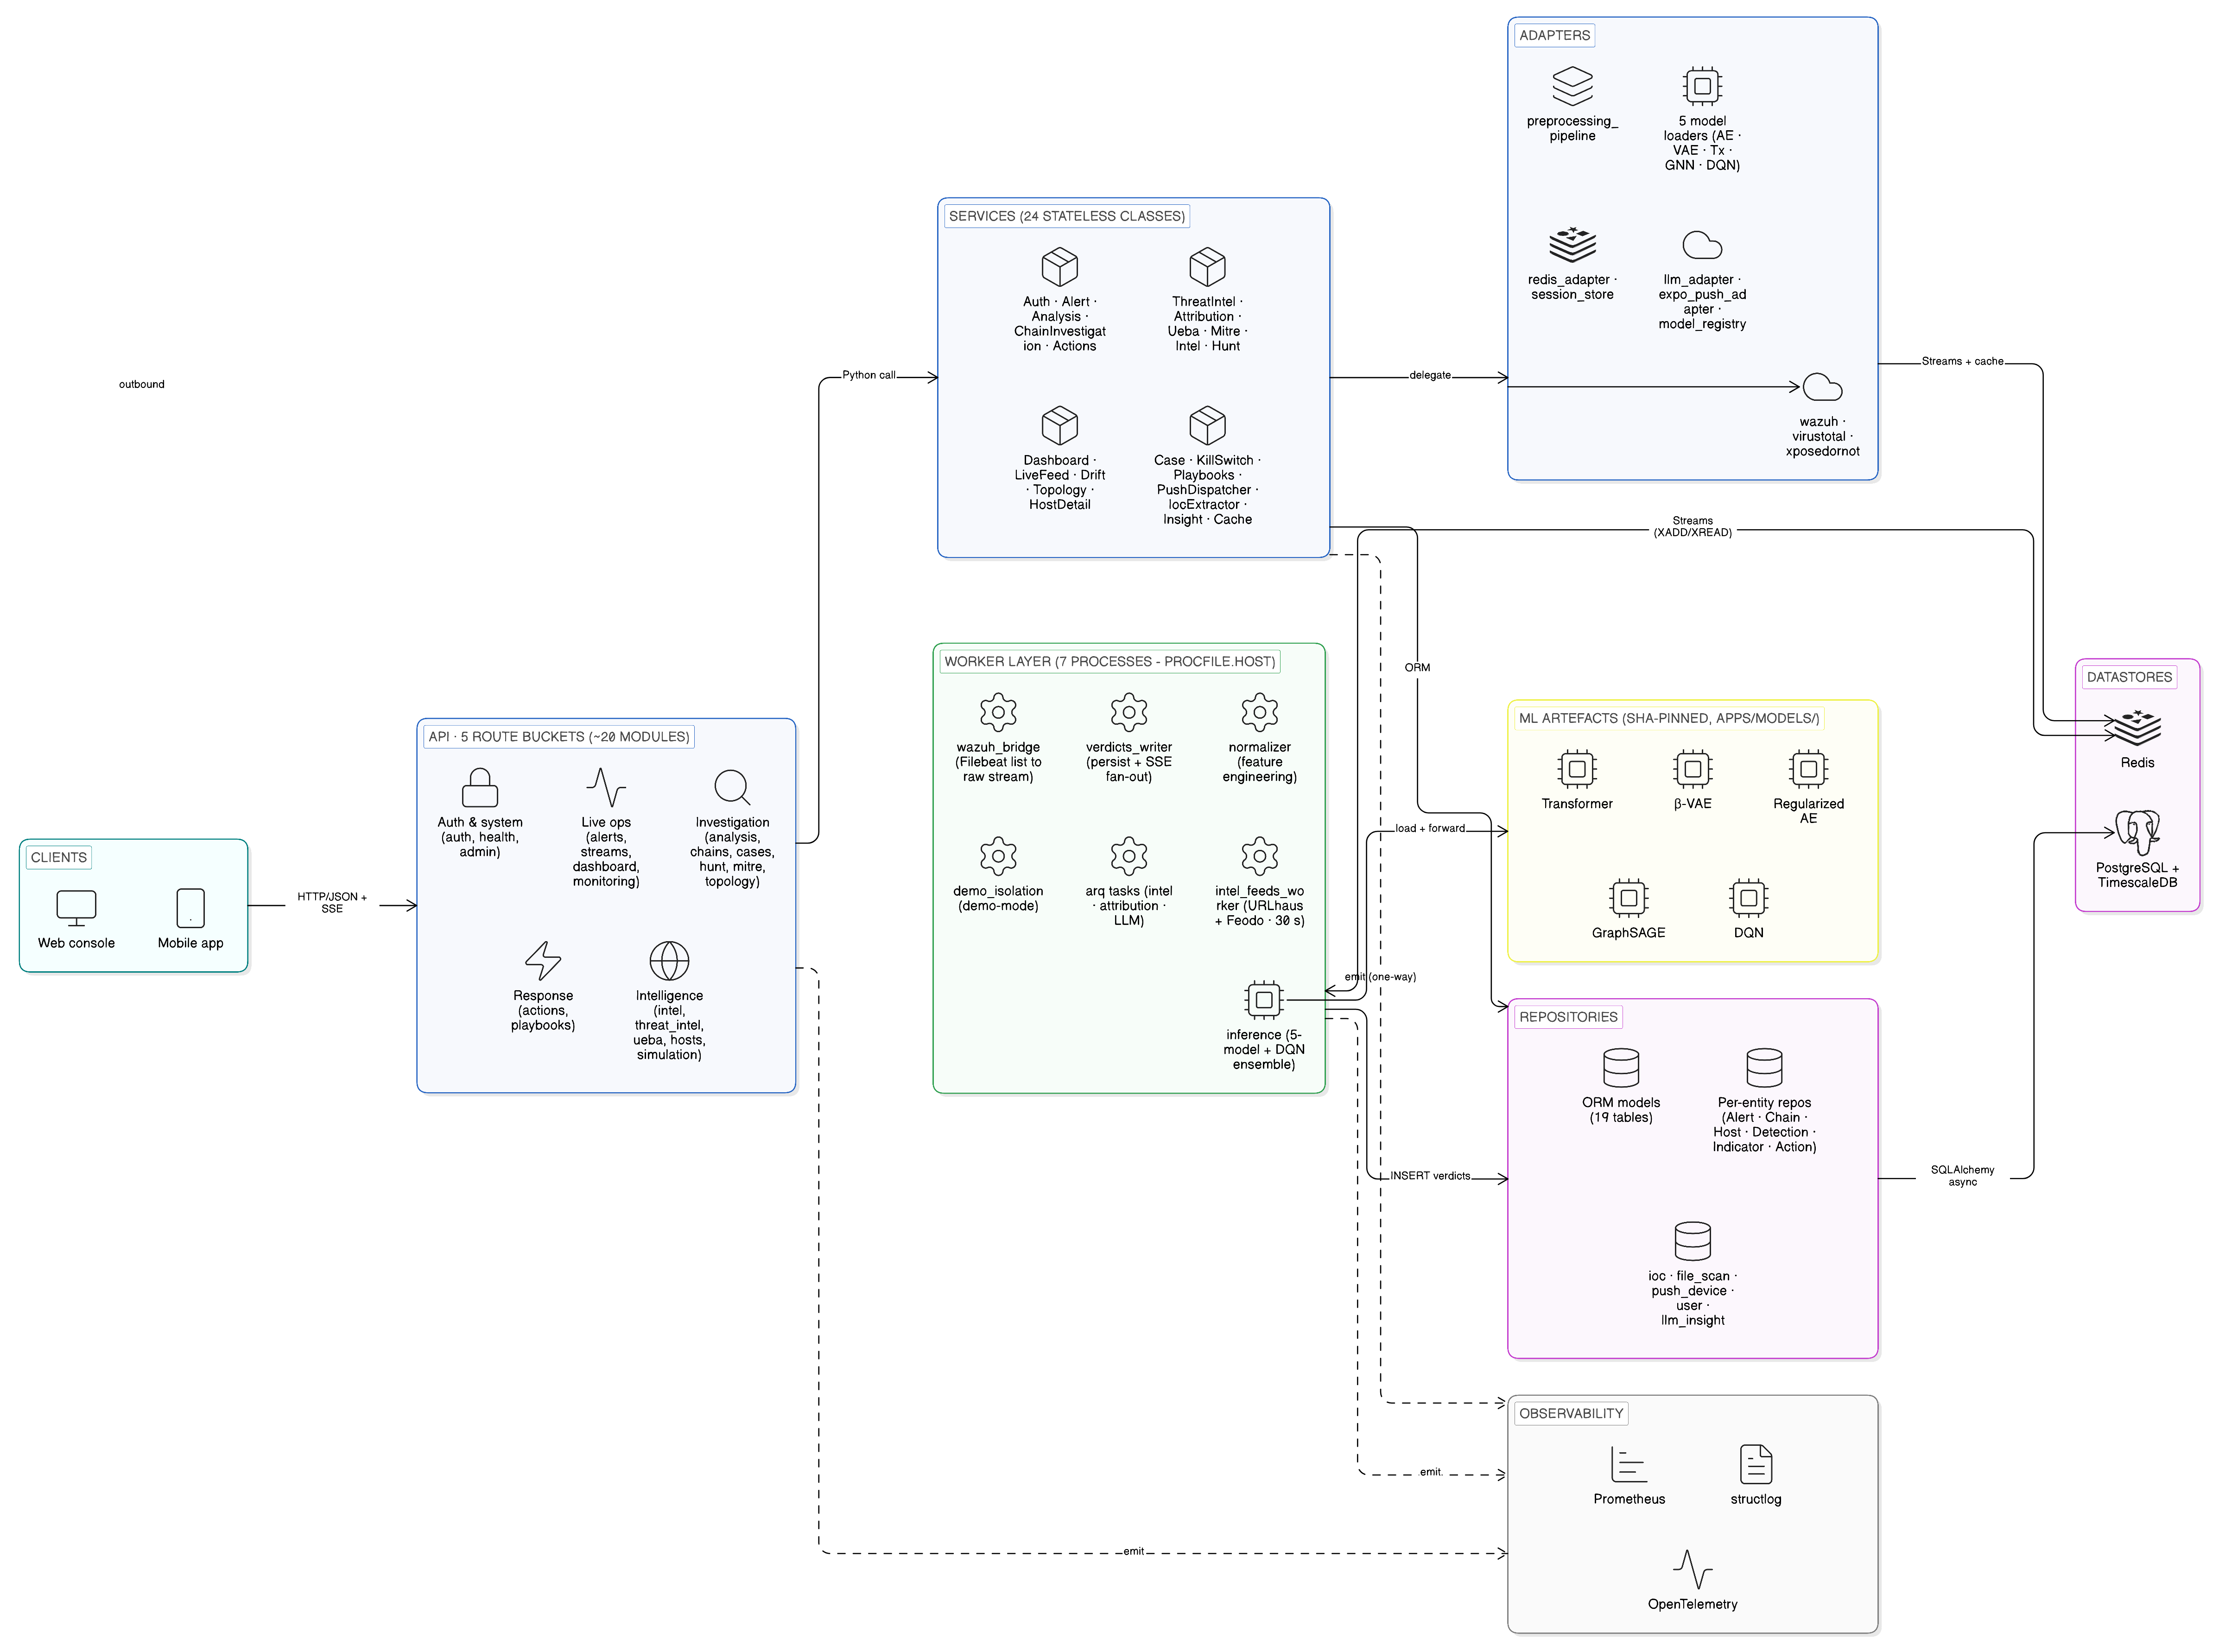
\includegraphics[width=0.95\textwidth]{figures/ch4/diagrams/platform_components_internal}
  \caption{Backend engineering decomposition of CAVIX.}
  \label{fig:ch4:components}
  \par\medskip
  As figure~\ref{fig:ch4:components} shows, the diagram inventories the FastAPI route buckets (auth, live-ops, investigation, response, intelligence), the 24 stateless service classes grouped by domain, the repository layer that wraps the 19 ORM tables, the adapter layer that isolates external dependencies (model loaders, preprocessing, external APIs, Redis, AI clients), the seven worker processes managed through \texttt{Procfile.host}, the five SHA-pinned model artefacts under \texttt{apps/models/}, and the observability stack (structlog, Prometheus, OpenTelemetry). The four prose components of section~\ref{sec:platform-components} map across this picture: the Detection Engine corresponds to the inference worker plus model loaders plus the five model artefacts; the Wazuh Integration corresponds to \texttt{wazuh\_bridge} plus the Wazuh adapter; the Threat Intelligence Module corresponds to \texttt{intel\_feeds\_worker} plus the intel-domain services and routes; the Analyst Dashboard corresponds to the web and mobile clients plus the live-ops routes and services.
\end{figure}

\begin{figure}[H]
  \centering
  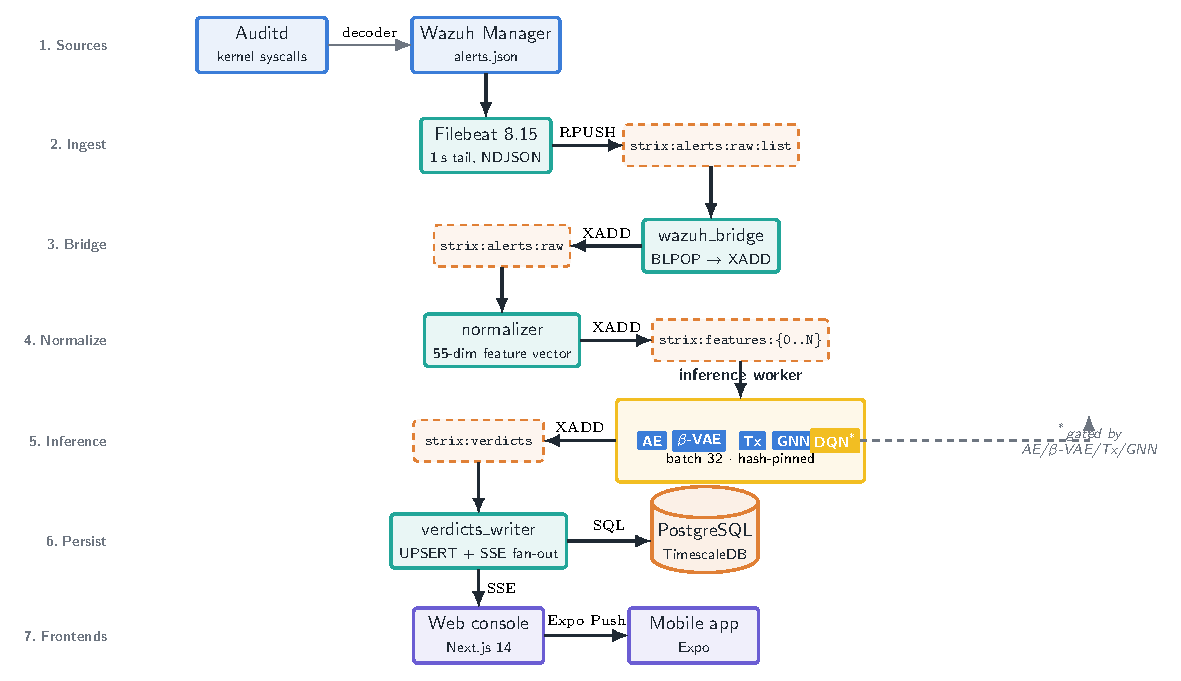
\includegraphics[width=\textwidth]{figures/ch4/diagrams/data_flow_master}
  \caption{The full data flow.}
  \label{fig:ch4:dataflowmaster}
  \par\medskip
  As shown in figure~\ref{fig:ch4:dataflowmaster}, stages are numbered on the left for reference in the rest of this section. Stream keys (orange dashed boxes) are Redis Streams \protect\cite{redis2024}; workers (green) are separate Python processes managed through \texttt{Procfile.host} or the Compose worker profile; the inference worker hosts the five-model ensemble. The DQN action is gated downstream by deterministic thresholds, marked with an asterisk and explained in figure~\ref{fig:ch4:dqngating}.
\end{figure}

\paragraph{Stage 1: Bridge.} The \texttt{wazuh\_bridge} worker is
intentionally tiny: it does a blocking \texttt{BLPOP} on the staging
list, wraps the raw JSON in a \texttt{RawAlertMessage} envelope, and
\texttt{XADD}s it onto the \texttt{strix:alerts:raw} stream. On any
failure during the \texttt{XADD}, it pushes the message back to the
head of the list so no event is lost. The bridge is the only
component where data loss is structurally possible (it is the single
point at which the staging list is consumed without an offset
mechanism), which is why we kept it as small as we could.

\paragraph{Stage 2: Normalize.} The \texttt{normalizer} consumes
the raw stream, builds the 55-dimensional feature vector through the
pipeline whose conceptual design is given in
chapter~\ref{chap:conception} and whose implementation lives under
\texttt{apps/normalizer/}, applies the canonical column ordering
listed in \texttt{selected\_features\_top25.json}, and writes a
\texttt{FeatureMessage} onto a shard of the
\texttt{strix:features:\{0..N\}} stream. The shard is chosen by a
SHA-1 of the agent ID modulo \texttt{INFERENCE\_NUM\_SHARDS}, which
gives us deterministic affinity per host (every alert from the same
agent lands on the same inference worker) while still allowing the
inference workers to scale horizontally. The shard count is
typically set to the number of CPU cores allocated to inference, so
that each worker is pinned to one core; below that, workers
under-utilise the host, and above it, the temporal locality the GNN
relies on starts to degrade.

\paragraph{Stage 3: Inference.} Each \texttt{inference} worker
listens on one shard. It loads all five model artefacts from
\texttt{apps/models/} on startup, and refuses to start at all if the
SHA-256 of any artefact does not match the registry. It batches up
to thirty-two events, runs them through the autoencoder, the
$\beta$-VAE, the Transformer and the GraphSAGE GNN, then feeds a
thirteen-dimensional state vector to the DQN. That state vector
concatenates four anomaly scores (autoencoder reconstruction error,
$\beta$-VAE malicious probability, Transformer next-stage confidence,
GraphSAGE node-risk score), seven one-hot indicators for the seven
non-zero CKC stages predicted by the Transformer, the current chain
length for the source host, and a normalised time-since-last-alert
counter. The five verdicts plus the chosen action are emitted as a
\texttt{VerdictMessage} onto the \texttt{strix:verdicts} stream.

\paragraph{Stage 4: Persist.} The \texttt{verdicts\_writer} batches
verdicts in five-second windows and persists them: an UPSERT on the
\texttt{hosts} table, INSERTs on \texttt{alerts} and the
\texttt{detections} hypertable, and an open-or-bump on the
\texttt{attack\_chains} table that groups consecutive alerts from the
same host into a single chain. The five-second window is the
shortest period over which the cost of preparing a batched
PostgreSQL INSERT amortises well across the verdict rate observed in
the lab (a few hundred per second under attack load), and it also
aligns with the refresh cadence of the dashboard's live tables, so
that the analyst sees a coherent batch rather than partial state.
Any DQN action that survives the gate is recorded in
\texttt{dqn\_actions} for the action-history view in the web
console.

\paragraph{Stage 5: Fan out.} The writer also publishes the verdict
on an SSE channel that the web console subscribes to. The mobile
client receives a push notification through Expo Push if, and only
if, the verdict's CKC stage is at or below S2 (Reconnaissance or
Weaponisation) and the gated DQN action is not \texttt{MONITOR}. The
S1--S2 cutoff is the result of an explicit cost--benefit choice: a
push notification only earns its place on the analyst's phone if it
arrives early enough to enable a response that prevents the next
stage of the kill chain. Alerts at S3 or later may still warrant
attention, but by then the chain forensic view on the web console is
the appropriate surface, not a mobile push.

The DQN gate is load-bearing. The ablation study in
chapter~\ref{chap:conception} shows that a pure-RL policy (one that
lets the DQN's chosen action propagate directly to the verdict)
produces a 100\,\% false-positive intervention rate on the lab's
benign traffic. The agent itself converged correctly on the synthetic
environment; the fix was to wrap its action rather than retrain it.

\begin{figure}[H]
  \centering
  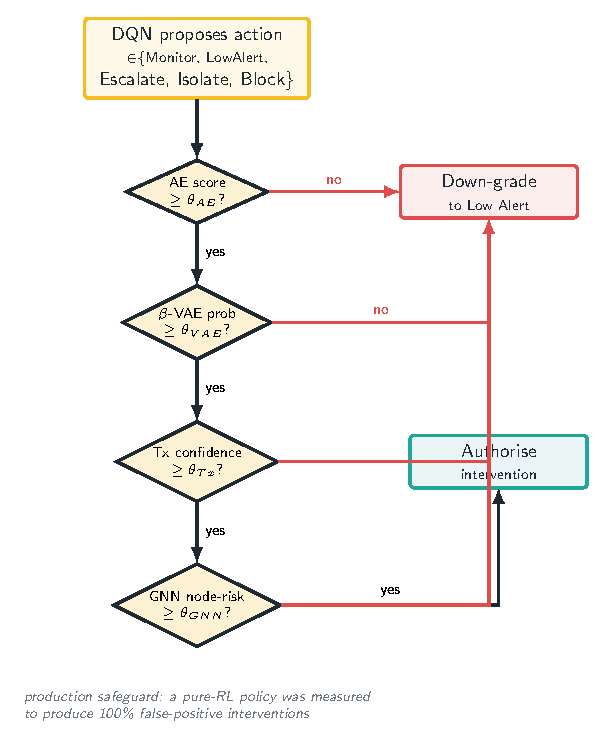
\includegraphics[width=0.62\textwidth]{figures/ch4/diagrams/dqn_gating_logic}
  \caption{The gating logic that wraps every DQN action.}
  \label{fig:ch4:dqngating}
  \par\medskip
  In figure~\ref{fig:ch4:dqngating}, an intervention (\texttt{ESCALATE}, \texttt{ISOLATE\_HOST}, \texttt{BLOCK\_USER\_IP}) is only authorised when all four deterministic checks (AE score, $\beta$-VAE probability, Transformer confidence and GNN node risk) exceed their thresholds. Any single failure down-grades the action to \texttt{LOW\_ALERT}.
\end{figure}

\subsection{Threat Intelligence Module}

The platform consumes two open-source CTI feeds: URLhaus
\cite{urlhaus2024} and the Feodo Tracker \cite{feodotracker2024},
both maintained by abuse.ch. The \texttt{intel\_feeds\_worker} polls
each feed every thirty seconds, deduplicates indicators by
\texttt{(indicator, type, source)}, and upserts the result into the
\texttt{intel\_indicators} table. The thirty-second interval is a
deliberate over-sample relative to abuse.ch's roughly minute-scale
publication cadence: under-sampling would risk missing the first
few seconds of an emerging indicator, while a tighter interval
yields no fresher data and only consumes connection capacity. The
poll cadence is exposed through the
\texttt{INTEL\_POLL\_INTERVAL\_SEC} environment variable so it can
be tuned if a future feed publishes more aggressively.

\begin{figure}[H]
  \centering
  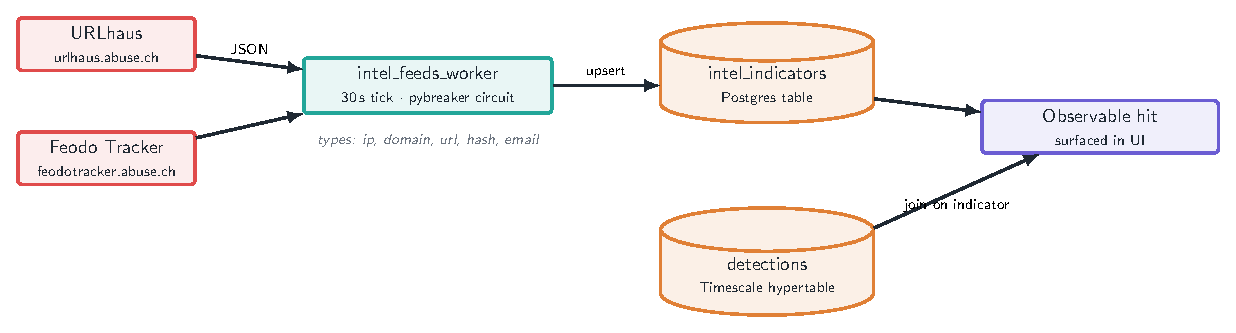
\includegraphics[width=0.9\textwidth]{figures/ch4/diagrams/threat_intel_schema}
  \caption{Threat-intelligence ingestion and the observable-hit surface.}
  \label{fig:ch4:intelschema}
  \par\medskip
  Figure~\ref{fig:ch4:intelschema} captures the following. URLhaus and Feodo Tracker indicators land in \texttt{intel\_indicators}; an internal alert is flagged as an "observable hit" the moment its IP, URL, domain or file hash matches any row in that table.
\end{figure}

Both feeds are wrapped in \texttt{pybreaker} circuit breakers. A
malformed response or a request that exceeds the ten-second
timeout opens the breaker for one minute, during which the worker
keeps serving stale indicators from the database and the operator
sees a small "degraded" badge on the Threat Intel tab. Both
durations are deliberate: the ten-second timeout is the
ninety-fifth-percentile response time we observed from abuse.ch
during steady-state operation, generous enough to ride out a slow
response without confusing transient latency with a feed outage;
the one-minute cool-down is the shortest interval after which the
feed is consistently observed to recover from the failure modes we
have seen (rate limiting, transient DNS errors), so retrying sooner
typically only re-trips the breaker. The worker is written to be
feed-agnostic, and adding a new source is a single function that
returns a list of indicator dictionaries.

\subsection{APT Early-Detection Dashboard}

The web console is the analyst's primary surface. Every page is
type-checked against the backend OpenAPI specification; every
expensive page is paginated. The four screenshots in this section
were captured during the writing of this chapter, against the same
running platform that produced the per-tactic report in
figure~\ref{fig:ch4:pertacticreport}.

\paragraph{Model Monitoring (AI Engine).}
The page directly under the "Model Monitoring" navigation entry
displays the five live models and the inference stream. The composite
F1 score is computed as the harmonic mean of the five test-set F1s
recorded at training time, exposed by the model registry; the
composite accuracy is the same idea applied to test-set accuracy.

\begin{figure}[H]
  \centering
  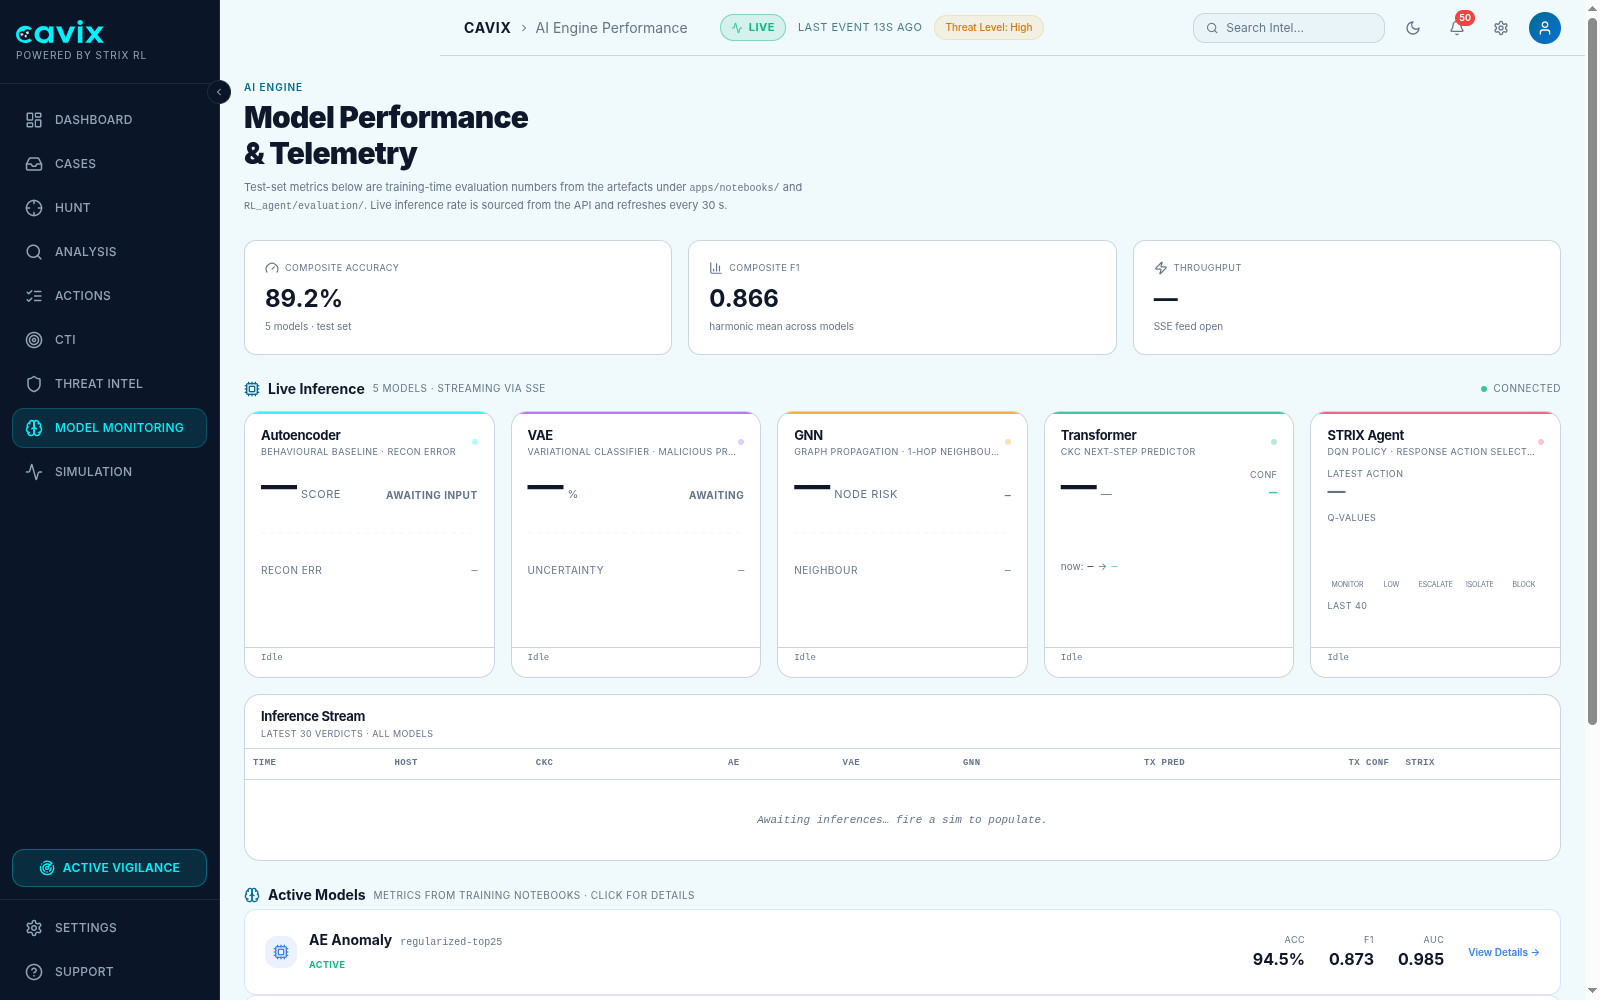
\includegraphics[width=0.95\textwidth]{figures/ch4/screenshots/dashboard_ai_engine}
  \caption{The Model Monitoring page.}
  \label{fig:ch4:dashAI}
  \par\medskip
  As illustrated in figure~\ref{fig:ch4:dashAI}, five model panels run along the top, each one displaying the live anomaly score or class probability as the model emits it. Underneath, the Inference Stream table is a live view of the most recent thirty verdicts.
\end{figure}

\paragraph{Attack Analysis (Chains).}
Clicking a chain opens a forensic report that reconstructs the chain's
stage timeline, the AI predictions per stage, the response playbook
that matched, and the most likely origin hypothesis (here APT28,
group identifier G0007 on MITRE ATT\&CK \cite{mitre_attack}).

\begin{figure}[H]
  \centering
  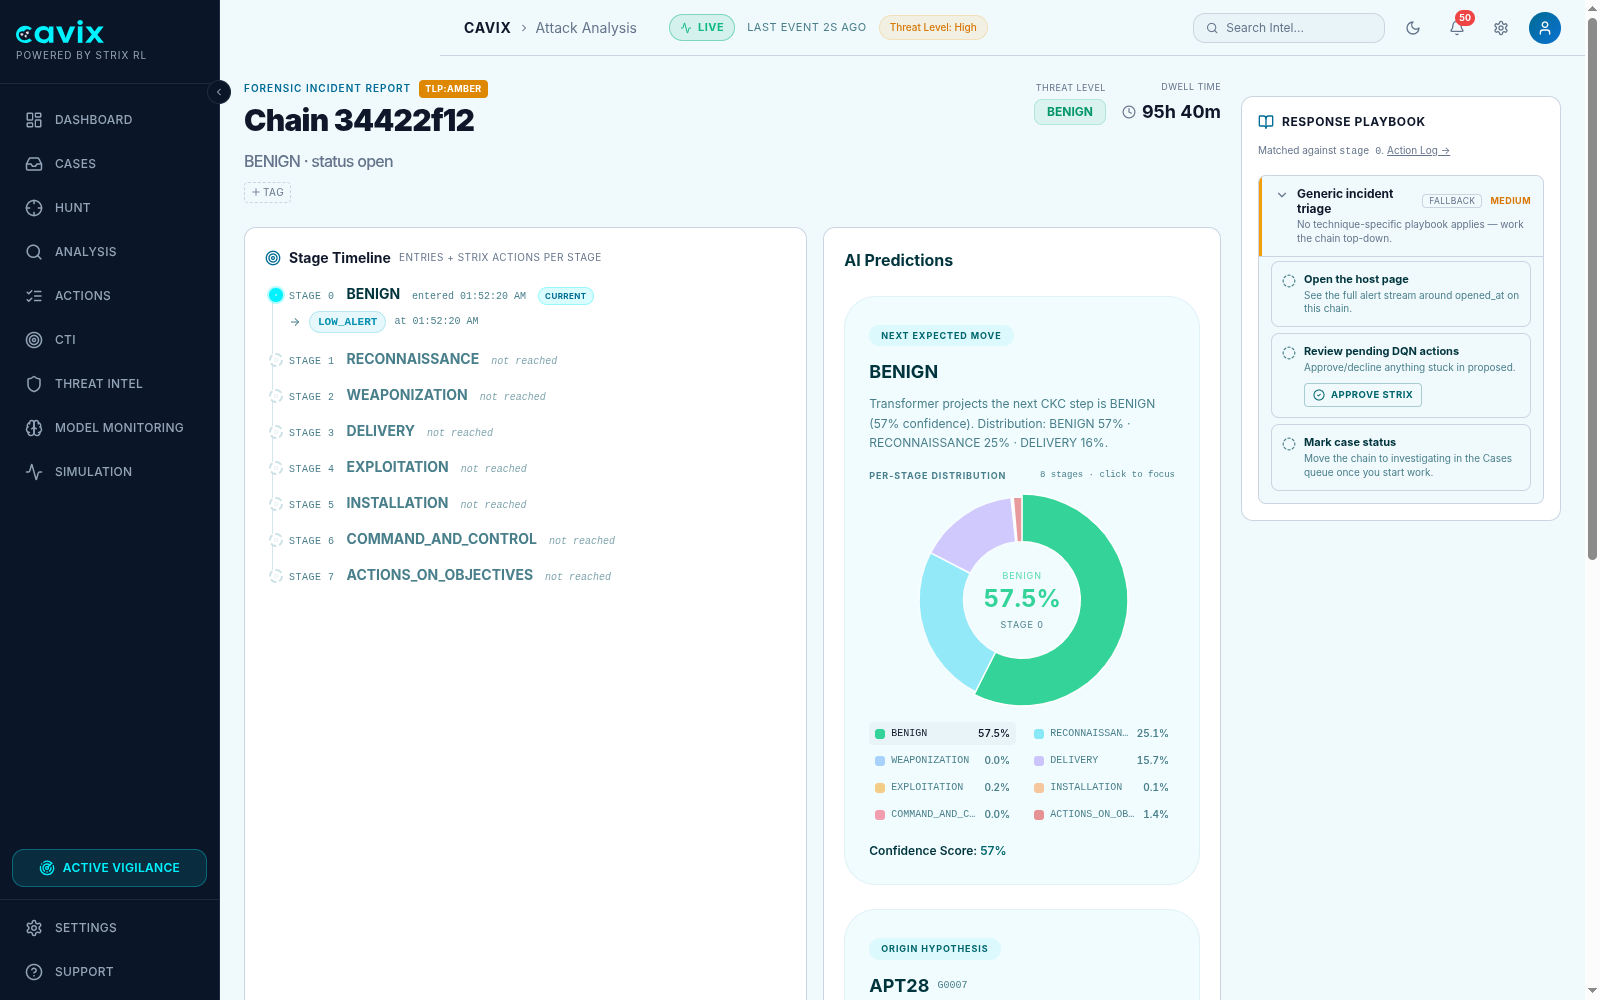
\includegraphics[width=0.95\textwidth]{figures/ch4/screenshots/dashboard_chains}
  \caption{The chain forensic report for an active investigation.}
  \label{fig:ch4:dashChains}
  \par\medskip
  As depicted in figure~\ref{fig:ch4:dashChains}, the donut on the right is the per-stage CKC distribution the Transformer predicted for this chain's next event; the Response Playbook on the far right is matched against the chain's current stage and the most recent DQN action.
\end{figure}

\paragraph{Topology.}
The Topology tab displays the live simulation graph: the attacker on
the left, the victims on the right, the tactics fired so far as
coloured chips above the graph. The right-hand panel is the GNN
Victim Graph, a separate visualization that overlays the GNN's
per-node risk score on top of the host inventory.

\begin{figure}[H]
  \centering
  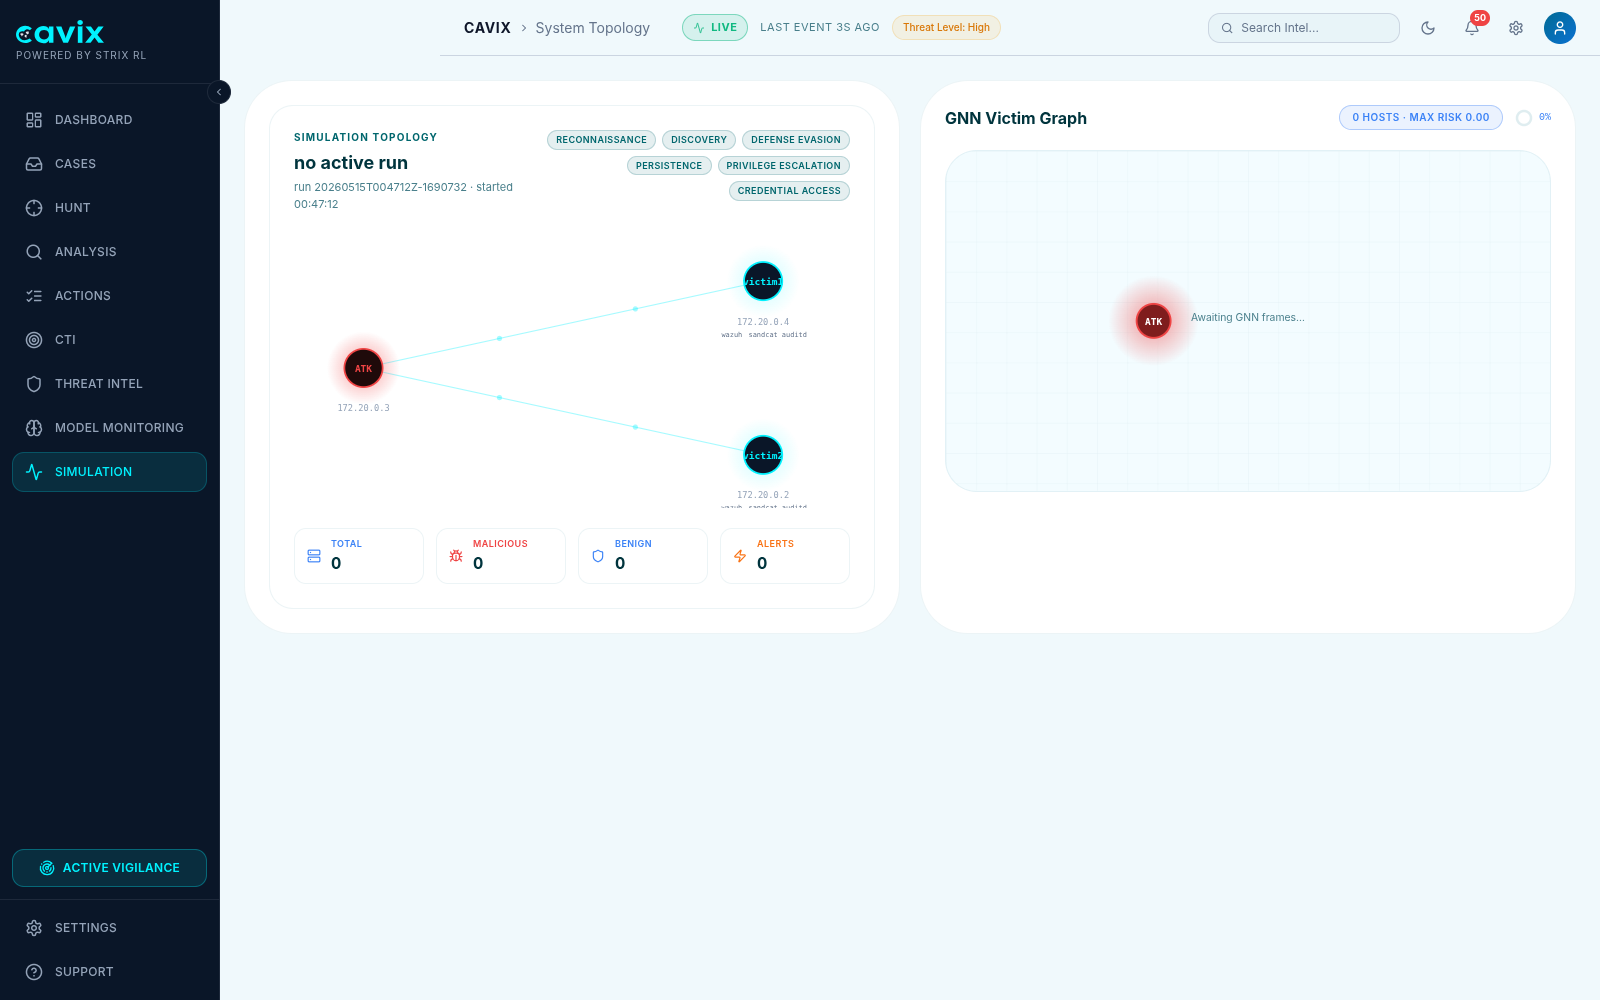
\includegraphics[width=0.95\textwidth]{figures/ch4/screenshots/dashboard_topology}
  \caption{The Topology tab during a paused run.}
  \label{fig:ch4:dashTopology}
  \par\medskip
  As figure~\ref{fig:ch4:dashTopology} shows, left: the simulation topology, sourced from the run manifest of figure \ref{fig:ch4:manifest}. Right: the GNN Victim Graph, currently awaiting fresh frames from the GraphSAGE layer.
\end{figure}

\paragraph{Mobile companion.}
The mobile application exposes a subset of the web functionality: the
vigilance feed (an SSE stream of verdicts), the chain detail page,
and a one-tap isolation control that re-uses the same gated DQN
action endpoint as the web console. Push notifications are routed
through Expo Push and are gated to S1 and S2 verdicts only.
Sending a phone notification for an S5 alert would be too late to be
useful, and would train the operator to mute the application.

\section{Conclusion}

This chapter walked through the concrete pieces of the CAVIX
platform that are required to make the conceptual framework of
chapter~\ref{chap:conception} executable: the dependencies and the
hardware budgets, the materialised form of the dataset inside the
system, the Caldera-driven lab that exercises the platform
end-to-end, and the ingestion, inference and fan-out path that turns
a raw Wazuh JSON line into a verdict on an analyst's screen. The
detailed dataset-selection rationale (section~\ref{sec:preprocessing})
and the feature-engineering pipeline that produces the 55-dimensional
vector remain to be documented in the next iteration of this
chapter.

A few engineering choices shaped the system more than others.
Hash-pinning every model artefact means we cannot accidentally deploy
a stale calibrator. Treating the OpenAPI specification as the single
source of truth means the web and mobile clients cannot drift away
from the backend without failing CI. The third, and the one whose
absence would have been hardest to detect, is the deterministic gate
wrapped around the DQN: without it, a pure-RL false positive could
reach production. None of these choices were obvious before the
corresponding incident; all of them are cheap to keep in place now.

Chapter~\ref{chap:evaluation} reuses the same stack to evaluate the platform. It
re-uses \texttt{lab\_simulate.sh}, the per-tactic report, and the
chain database introduced here to evaluate the platform under three
lenses: model-level metrics on the Karim dataset, RL-agent metrics on
the carved attack sequences, and system-level metrics (detection
latency, false-positive rate, end-to-end throughput) that only make
sense at the level of the whole pipeline.
